% !TeX root = ../thesis.tex

%%%%%%%%%%%%%%%%%%%%%%%%%%%%%%%%%%%%%%%%%%
\thesischapter[ch:microbiome][0.9\textwidth]
  {``Microbiome Datasets Are Compositional: And This Is Not Optional''}
  {--- G. B. Gloor, J. M. Macklaim, V. Pawlowsky-Glahn, and J. J. Egozcue, 2017}
  {Microbiome data as statistical objects}
\nocite{gloor2017microbiome}
\chapterabstract{This chapter formalizes microbiome sequencing data as statistical objects and describes the structural properties that shape downstream analyses. It introduces how sequencing experiments give rise to count matrices and discusses why compositionality, sparsity, heterogeneous library sizes, overdispersion, and high dimensionality challenge standard statistical methods. The chapter then reviews key preprocessing choices, including aggregation, filtering, library-size adjustment, zero handling, and transformation, and discusses their implications for downstream inference.}
\chaptercontents
%%%%%%%%%%%%%%%%%%%%%%%%%%%%%%%%%%%%%%%%%%

%%%%%%%%%%%%%%%%%%%%%%%%%%%%%%%%%%%%%
\section{Introduction}
\label{sec:2micro:introduction}
%%%%%%%%%%%%%%%%%%%%%%%%%%%%%%%%%%%%%

Microbiome sequencing experiments produce data that are biologically rich yet statistically constrained. Before turning to specific analysis targets, it is therefore necessary to clarify what kind of mathematical objects microbiome data represent and which structural properties characterize them. This chapter formalizes microbiome count data as high-dimensional, compositional, and sparse data objects arising from complex sampling processes. We begin by outlining how sequencing technologies give rise to count matrices and associated metadata. We then examine the key statistical characteristics of these data, including compositionality, library size variability, sparsity, overdispersion, and high dimensionality. Finally, we discuss common preprocessing steps and their implications for downstream analysis. The purpose of this chapter is not to introduce new methodology, but to establish the statistical and geometric foundations on which the analyses and methodological developments in later chapters are built.

%%%%%%%%%%%%%%%%%%%%%%%%%%%%%%%%%%%%%
\section{From sequencing reads to count matrices}
\label{micro:count_data}
%%%%%%%%%%%%%%%%%%%%%%%%%%%%%%%%%%%%%

High-throughput sequencing technologies enable the culture-independent characterization of microbial communities across diverse environments \citep{caporaso2012ultrahighthroughput,shendure2017dna}. In microbiome research, two principal strategies are commonly employed. Marker-gene amplicon sequencing targets specific conserved genomic regions to infer taxonomic composition, whereas shotgun metagenomic sequencing fragments and sequences a broad collection of DNA fragments extracted from a sample, thereby providing information on both taxonomic composition and functional potential \citep{sharpton2014introduction,quince2017shotgun}.

In bacterial and archaeal studies, marker-gene approaches most commonly target the 16S ribosomal RNA (rRNA) gene \citep{sanschagrin2014nextgeneration}. The 16S rRNA gene encodes a structural component of the small ribosomal subunit and is universally present in prokaryotes. Its sequence consists of highly conserved regions interspersed with hypervariable regions. The conserved regions enable the design of universal primers for polymerase chain reaction (PCR) amplification, while the variable regions accumulate mutations that reflect evolutionary divergence and thus provide taxonomic information \citep{chakravorty2007detailed}. The phylogenetic relevance of rRNA sequences and their role in reconstructing evolutionary relationships were systematically established by \citet{woese1987bacterial}, laying the foundation for modern microbial taxonomy. For fungal communities, the internal transcribed spacer (ITS) region serves as a widely accepted marker due to its higher interspecific variability \citep{schoch2012nuclear}, while the 18S rRNA gene is frequently used for eukaryotic microorganisms \citep{hadziavdic2014characterization}.

A fundamental characteristic of standard marker-gene sequencing protocols is that they produce relative rather than absolute abundance measurements. Because sequencing depth is finite and the total number of reads per sample is limited, the observed counts reflect the proportion of sequencing effort allocated to each taxon rather than their actual microbial load \citep{gloor2017microbiome}. 

To address this limitation, quantitative microbiome profiling protocols have been proposed. These approaches either estimate total microbial load independently, for example via flow cytometry \citep{props2017absolute,vandeputte2017quantitative}, or introduce known internal standards prior to sequencing to enable calibration of observed counts \citep{lin2019quantitative,stammler2016adjusting}. While such strategies can provide valuable information on absolute microbial abundance, many microbiome datasets remain based solely on sequencing counts without independent absolute quantification.

Shotgun metagenomic sequencing differs from marker-gene sequencing in that it does not target a specific genomic region but instead sequences a broad collection of DNA fragments extracted from a sample. As a result, shotgun approaches allow simultaneous taxonomic and functional profiling at higher resolution \citep{quince2017shotgun}. Nevertheless, standard shotgun protocols also yield read counts constrained by total sequencing depth and therefore share the compositional characteristics of marker-gene data unless complemented by independent absolute quantification.

In this thesis, we primarily focus on marker-gene sequencing data, in particular 16S rRNA amplicon sequencing, which remains one of the most widely used approaches in host-associated microbiome research. The statistical challenges arising from compositional constraints, sparsity, and high dimensionality are prominent in such datasets, making them a natural setting for methodological development. Many of the inferential principles discussed later, however, extend to shotgun metagenomic data as well.

After bioinformatic preprocessing, sequencing reads are summarized into features. In amplicon sequencing workflows, this commonly includes quality control, denoising, and chimera removal. Depending on the bioinformatic pipeline, these features may correspond to amplicon sequence variants (ASVs), which resolve sequences at single-nucleotide resolution \citep{callahan2016dada2}, to operational taxonomic units (OTUs), or to genes or taxonomic groups at a specified rank. 

The resulting data are organized into a count matrix. 
In this thesis, $n$ denotes the number of samples and $p$ the number of taxa (features), so that the count matrix is defined as
\begin{equation}
\label{eq:micro:count_matrix}
    \mathbf{X} = (x_{ki}) \in \mathbb{N}_0^{n \times p}, 
    \quad k = 1, \dots, n, \; i = 1, \dots, p.
\end{equation}
Here, $x_{ki}$ denotes the number of reads assigned to taxon $i$ in sample $k$. 
The total number of reads observed in sample $k$,
\begin{equation}
	\label{eq:micro:library_size}
    m_k = \sum_{i=1}^{p} x_{ki},
\end{equation}
is commonly referred to as the \emph{library size}. 
In the microbiome literature, the term \emph{sequencing depth} is often used synonymously. 
Strictly speaking, sequencing depth refers to the intensity of sequencing effort applied to a sample, whereas library size denotes the realized total number of reads obtained. 
In this thesis, we use the term \emph{library size} to emphasize that $m_k$ is an observed data quantity.

In addition to the count matrix, microbiome studies typically include two further data components. 
First, a sample metadata table contains clinical, environmental, or \text{experimental} covariates for each sample, such as age, treatment group, or sampling location. 
Second, each feature (taxon) is accompanied by a taxonomic annotation that assigns it to hierarchical ranks such as phylum, class, order, family, genus, and species. 
This taxonomic table reflects the biological classification derived from sequence similarity or reference databases and enables aggregation of counts at different taxonomic levels.

The count matrix $\mathbf{X} \in \mathbb{N}_0^{n \times p}$ constitutes the primary statistical object underlying microbiome data analysis. Its properties are fundamentally shaped by the sequencing process, the aggregation of reads into features, and the compositional constraint imposed by finite library sizes. While the count matrix forms the basis for most quantitative analyses, metadata and taxonomic structure play a crucial role in interpretation, aggregation, and group comparisons.

%%%%%%%%%%%%%%%%%%%%%%%%%%%%%%%%%%%%%
\section{Characteristics of microbiome data}
\label{sec:2micro:characteristics}
%%%%%%%%%%%%%%%%%%%%%%%%%%%%%%%%%%%%%

\begin{figure}[H]
\centering
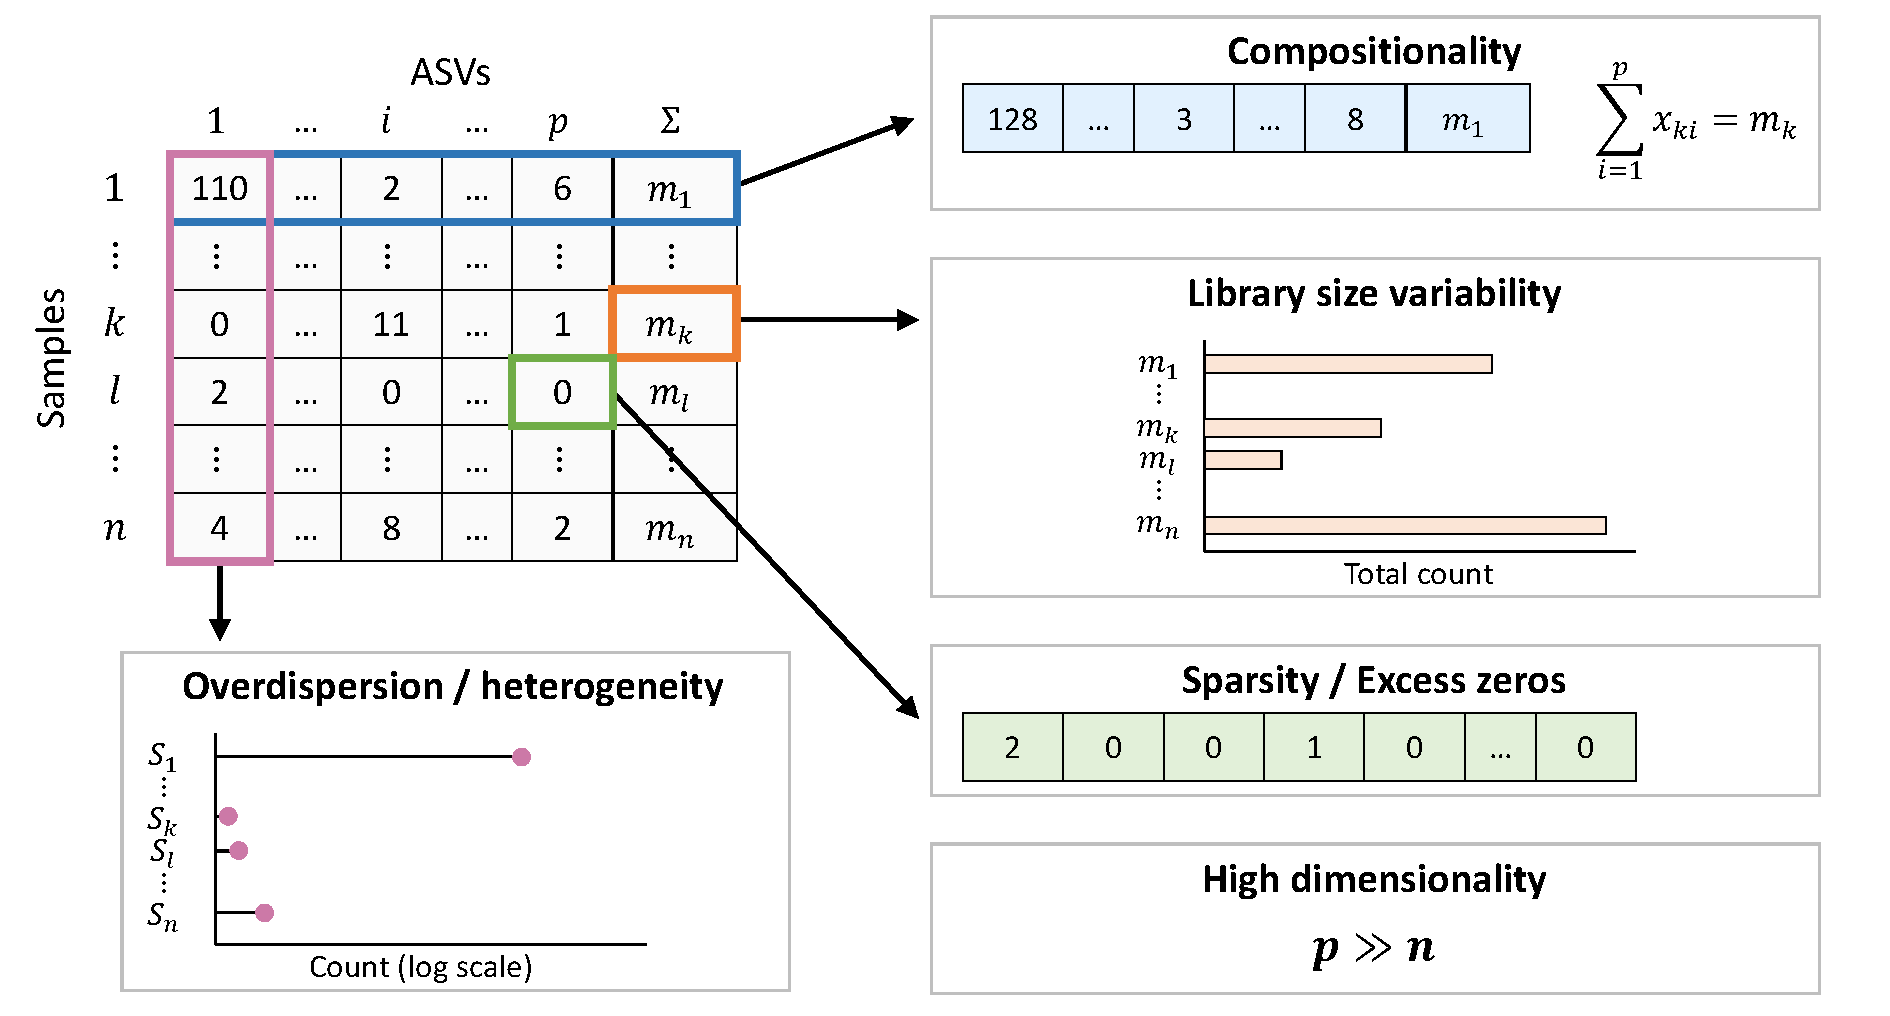
\includegraphics[width=\textwidth]{../ch02_microbiome_data/overview_figures/overview_characteristics.pdf}
\caption{\textbf{Overview of characteristic properties of microbiome count data.} The count matrix contains non-negative read counts for $n$ samples and $p$ taxa. Each sample is constrained by its library size $m_k$, leading to compositional structure. Library sizes vary across samples, many taxa contain zero counts, count distributions may be highly heterogeneous and overdispersed, and the number of taxa is often large relative to the number of samples. These properties motivate the preprocessing and modeling choices discussed throughout this chapter.}
\label{fig:2micro:overview_characteristics}
\end{figure}

Microbiome count matrices have several structural properties that distinguish them from unconstrained multivariate data matrices. These properties arise from the sequencing process, the aggregation of reads into microbial features, and the ecological structure of microbial communities. Figure~\ref{fig:2micro:overview_characteristics} provides an overview of the main characteristics discussed in this section. The entries of the count matrix are constrained by the sample-specific library size, library sizes vary between samples, many entries are zero, count distributions are heterogeneous and overdispersed, and the number of taxa is often large relative to the number of samples. Each of these aspects affects how microbiome data should be preprocessed, modeled, and interpreted.

%====================================
\subsection{Compositionality and induced dependence}
\label{sec:2micro:charact:compositionality}
%====================================

A defining structural property of microbiome sequencing data is their \emph{compositional} nature. 
Under typical high-throughput sequencing protocols, only a finite number of reads can be obtained from each sample \citep{gloor2017microbiome}. 
For each sample $k$, the total number of reads
\begin{equation}
    m_k = \sum_{i=1}^{p} x_{ki}
\end{equation}
is determined primarily by technical and experimental factors such as sequencing platform capacity, degree of multiplexing, PCR amplification efficiency, and DNA extraction efficiency, rather than by the absolute microbial load in the underlying biological environment \citep{nearing2021identifying}. 
Consequently, the observed counts $x_{ki}$ reflect the relative allocation of sequencing effort across taxa rather than their absolute abundances.

Conditional on the sample-specific library size $m_k$, the count vector $\mathbf{x}_k = (x_{k1}, \dots, x_{kp})^\top$ satisfies the constant-sum constraint
\begin{equation}
\sum_{i=1}^{p} x_{ki} = m_k,
\end{equation}
which restricts it to a $(p-1)$-dimensional affine subspace of $\mathbb{R}^{p}$.
This restriction is referred to as \emph{closure} and forms the foundation of compositional data analysis \citep{aitchison1982statistical,gloor2016its}. 
Importantly, closure is induced by the sampling mechanism itself and does not result from any subsequent normalization procedure.

Closure implies that the components of $\mathbf{x}_k$ cannot vary independently. 
Conditional on $m_k$, an increase in one component must be accompanied by a decrease in at least one other component, even if the corresponding taxa are biologically unrelated.
As a result, the count vector is identifiable only up to a positive scaling factor: absolute abundances cannot be recovered from sequencing data without additional external information. 
Inference is therefore restricted to relative quantities.

From a statistical perspective, compositionality implies that standard multivariate methods developed for unconstrained Euclidean data cannot be applied without modification. 
Because the components of $\mathbf{x}_k$ satisfy a linear constraint, the data exhibit inherent dependence induced by the constant-sum restriction. 
In particular, naive covariance and correlation estimates computed directly from raw counts may reflect this structural dependence rather than genuine biological associations. 
Thus, apparent negative correlations between taxa may arise purely as a mathematical consequence of closure rather than genuine biological interaction.

To address these issues, Aitchison developed a principled framework for the statistical analysis of compositional data based on log-ratio transformations \citep{aitchison1982statistical}. 
The central insight is that only relative information between components is meaningful in the presence of closure, and that this information is naturally captured by ratios between components. 
Log-ratio transformations embed compositional vectors into a $(p-1)$-dimensional Euclidean space, thereby enabling the application of conventional multivariate techniques while respecting the relative nature of the data.

Aitchison’s framework is grounded in two fundamental principles. 
The first is \emph{scale invariance}: statistical conclusions should remain unchanged under multiplication of all components of a composition by a positive constant, reflecting the fact that only relative information is observable. 
The second is \emph{subcompositional coherence}, which requires that inference based on a subset of components be consistent with that obtained from the full composition restricted to the same subset. 
These principles formalize the idea that compositional data carry only relative information and that analyses should not depend on arbitrary changes in total scale or on the presence of additional irrelevant components \citep{aitchison1982statistical,greenacre2023aitchisons}.

However, log-ratio transformations require strictly positive components, which is problematic in the presence of zero counts. 
The interplay between compositional structure and sparsity therefore introduces additional theoretical and methodological challenges that are discussed in the subsequent sections.

%====================================
\subsection{Library size variability}
\label{sec:2micro:charact:librarysize}
%====================================

While closure describes a within-sample constraint, the total number of counts varies considerably across samples within the same study. 
As introduced above, the library size
\[
m_k = \sum_{i=1}^{p} x_{ki}
\]
is primarily determined by technical and experimental factors rather than by the absolute microbial load in the biological specimen. In practice, the values $m_k$ often differ substantially across samples.

Causes for library size variability include differences in DNA extraction efficiency, amplification yield during polymerase chain reaction, sample multiplexing, and stochastic fluctuations during library preparation \citep{nearing2021identifying}. 
As a result, two samples with identical underlying community composition may exhibit different total read counts purely due to technical variation.

This heterogeneity has important statistical consequences. 
First, raw counts are not directly comparable across samples: even when two samples share identical underlying community composition, the sample with larger library size will produce larger observed counts. 
Differences in $m_k$ can therefore induce apparent differences in taxon abundances that are unrelated to biological variation.

\newpage
Second, sampling variability depends on library size. 
Samples with smaller library sizes provide less information about low-abundance taxa and are more prone to sampling zeros. 
Thus, the library size influences the resolution at which community composition is observed and interacts with sparsity and the occurrence of sampling zeros.

In many sequencing studies, library size is primarily a technical quantity that affects the scale and variability of observed counts. Unless independently calibrated, it should therefore not be interpreted directly as a measure of biological abundance.
Statistical analyses must therefore account for heterogeneous library size to avoid confounding biological differences with differences in sequencing effort. 
Approaches for handling library size variability are discussed in the preprocessing section.


%====================================
\subsection{Sparsity and excess zeros}
\label{sec:2micro:charact:sparsity}
%====================================

Beyond compositionality and heterogeneous library sizes, microbiome count data are characterized by pronounced sparsity and a high prevalence of zero counts. 
In typical datasets, a substantial proportion of entries in the count matrix $\mathbf{X}$ are equal to zero.

Sparsity reflects both the ecological structure of microbial communities and limitations of the measurement process.
Abundance distributions are typically highly uneven: a small number of taxa account for a large fraction of the total reads, whereas many taxa occur at low abundance or only in a subset of samples. 
Consequently, the empirical distribution of counts is strongly right-skewed, and rare taxa contribute disproportionately to the number of zero entries \citep{xia2024applied,li2015microbiome}.

Observed zeros in microbiome data are heterogeneous and may arise through different mechanisms. 
Following terminology from compositional data analysis \citep{martin-fernandez2003dealing,martin2011dealing,filzmoser2018applied}, one may distinguish:

\begin{itemize}
    \item \emph{Structural zeros}, corresponding to true absence of a taxon in a given environment;
    \item \emph{Rounded zeros}, where a taxon is present at very low abundance but is not detected by the measurement process;
    \item \emph{Sampling zeros}, which arise because sequencing produces a finite random sample of reads, so that taxa with low underlying abundance may not be observed in a given sample.
\end{itemize}

While these mechanisms differ conceptually, they cannot be distinguished from the observed count matrix alone. 
In practice, many zeros reflect a combination of low underlying abundance and finite sampling depth, particularly in samples with small library sizes.

From a statistical perspective, sparsity and excess zeros have several important implications. 
First, they complicate transformations and modeling strategies that require strictly positive values, such as log-ratio representations. 
Second, taxa observed in only a small subset of samples contribute limited information for the estimation of means, variances, or pairwise associations. 
For rare taxa, the number of samples contributing informative non-zero observations can be substantially smaller than the nominal sample size $n$ \citep{kurtz2015sparse}, leading to increased estimator variability and reduced stability in downstream analyses.

Moreover, sparsity interacts with compositionality and library size variability. 
Low-abundance taxa are particularly sensitive to fluctuations in sequencing depth and are more prone to sampling zeros, amplifying apparent differences across samples. 
As a result, preprocessing decisions such as filtering rare taxa or handling zeros can have substantial influence on subsequent statistical inference.

%====================================
\subsection{Overdispersion and heterogeneity}
\label{sec:2micro:charact:overdispersion}
%====================================

In addition to sparsity and excess zeros, microbiome count data typically exhibit substantial variability across samples that exceeds what would be expected under simple count models. 
This phenomenon is commonly referred to as \emph{overdispersion} \citep{xia2024applied,weiss2017normalization}.

Classical models for count data provide a useful reference point. 
Under an independent Poisson model, the variance of each taxon count equals its mean. 
Similarly, under a multinomial sampling model conditional on the library size $m_k$, the variance structure is fully determined by $m_k$ and the underlying relative abundances. 
Both formulations imply a restrictive relationship between mean and variance.

Empirical microbiome data frequently exhibit variability that exceeds the variance implied by simple Poisson or multinomial sampling models with fixed underlying abundance parameters. 
Even after accounting for library size, the observed variability of taxon counts across samples often exceeds that predicted by Poisson or multinomial sampling models with fixed underlying abundance parameters.
This additional variability may reflect heterogeneity in underlying relative abundances across samples, arising from biological variation, technical effects, or both \citep{weiss2017normalization,xia2024applied}.

Ignoring overdispersion can lead to underestimated variance, anticonservative hypothesis tests, and inflated false positive rates \citep{anders2010differential,robinson2010edger}. In high-dimensional settings, heterogeneous variance structures further complicate covariance and association estimation, particularly for low-abundance taxa.

To accommodate overdispersion, models with explicit dispersion parameters, such as negative binomial or Dirichlet-multinomial formulations, are commonly employed. 
Alternatively, variance-stabilizing transformations may be applied prior to downstream analysis. 
The choice of strategy depends on the inferential objective and is discussed in later sections.

%====================================
\subsection{High dimensionality}
\label{sec:2micro:charact:highdim}
%====================================

Microbiome feature tables, particularly at fine taxonomic resolution, often contain a large number of taxa $p$ relative to the number of samples $n$, resulting in the so-called ``large $p$, small $n$'' regime \citep{xia2024applied}. In this setting, classical statistical procedures developed for the $p<n$ regime are no longer directly applicable.

When $p$ is comparable to or exceeds $n$, empirical covariance matrices become singular or ill-conditioned, and least-squares estimators are either non-unique or exhibit high variance. 
Regression models, multivariate hypothesis tests, and dimension-reduction techniques may therefore become unstable without additional structural assumptions or regularization.

High dimensionality also increases the burden of multiple testing at the feature level and inflates the number of potential pairwise relationships when studying dependence structures. 
As a consequence, statistical inference in microbiome studies typically requires penalization, dimension reduction, or other regularized approaches tailored to high-dimensional data.

Taken together, compositionality, heterogeneous library sizes, sparsity, overdispersion, and high dimensionality define a statistical regime that differs fundamentally from classical multivariate data settings and requires a dedicated statistical methodology.

%====================================
\subsection{Consequences for statistical analysis}
\label{sec:2micro:charact:consequences}
%====================================

The structural properties discussed above are not merely technical nuisances but fundamentally shape the geometry of the sample space and the validity of downstream analyses. Compositionality implies that observations reside in the simplex rather than in unconstrained Euclidean space \citep{aitchison1986statistical}, sparsity gives rise to highly skewed count distributions with many zero observations, and high dimensionality challenges classical statistical procedures when the number of features is comparable to or exceeds the number of samples, leading, for instance, to unstable covariance estimation and non-unique unregularized regression estimates \citep{xia2024applied}.

Taken together, these characteristics restrict the applicability of standard parametric modeling strategies and complicate the construction of reliable reference distributions for hypothesis testing. They affect all three analysis targets considered in this thesis: community-level summaries, feature-level measures, and association networks. In comparative analyses, resampling-based procedures such as permutation tests therefore become attractive whenever analytic null distributions are unavailable or unreliable, provided that the permutation scheme is compatible with the study design and the null hypothesis. However, as discussed in Chapter~\ref{ch:permapprox}, permutation testing also has intrinsic limitations under finite computational budgets. The statistical developments of this thesis therefore originate directly from the structural constraints formalized in the present chapter.

%%%%%%%%%%%%%%%%%%%%%%%%%%%%%%%%%%%%%
\section{Taxonomic aggregation}
\label{sec:2micro:aggregation}
%%%%%%%%%%%%%%%%%%%%%%%%%%%%%%%%%%%%%

\begin{figure}[H]
\centering
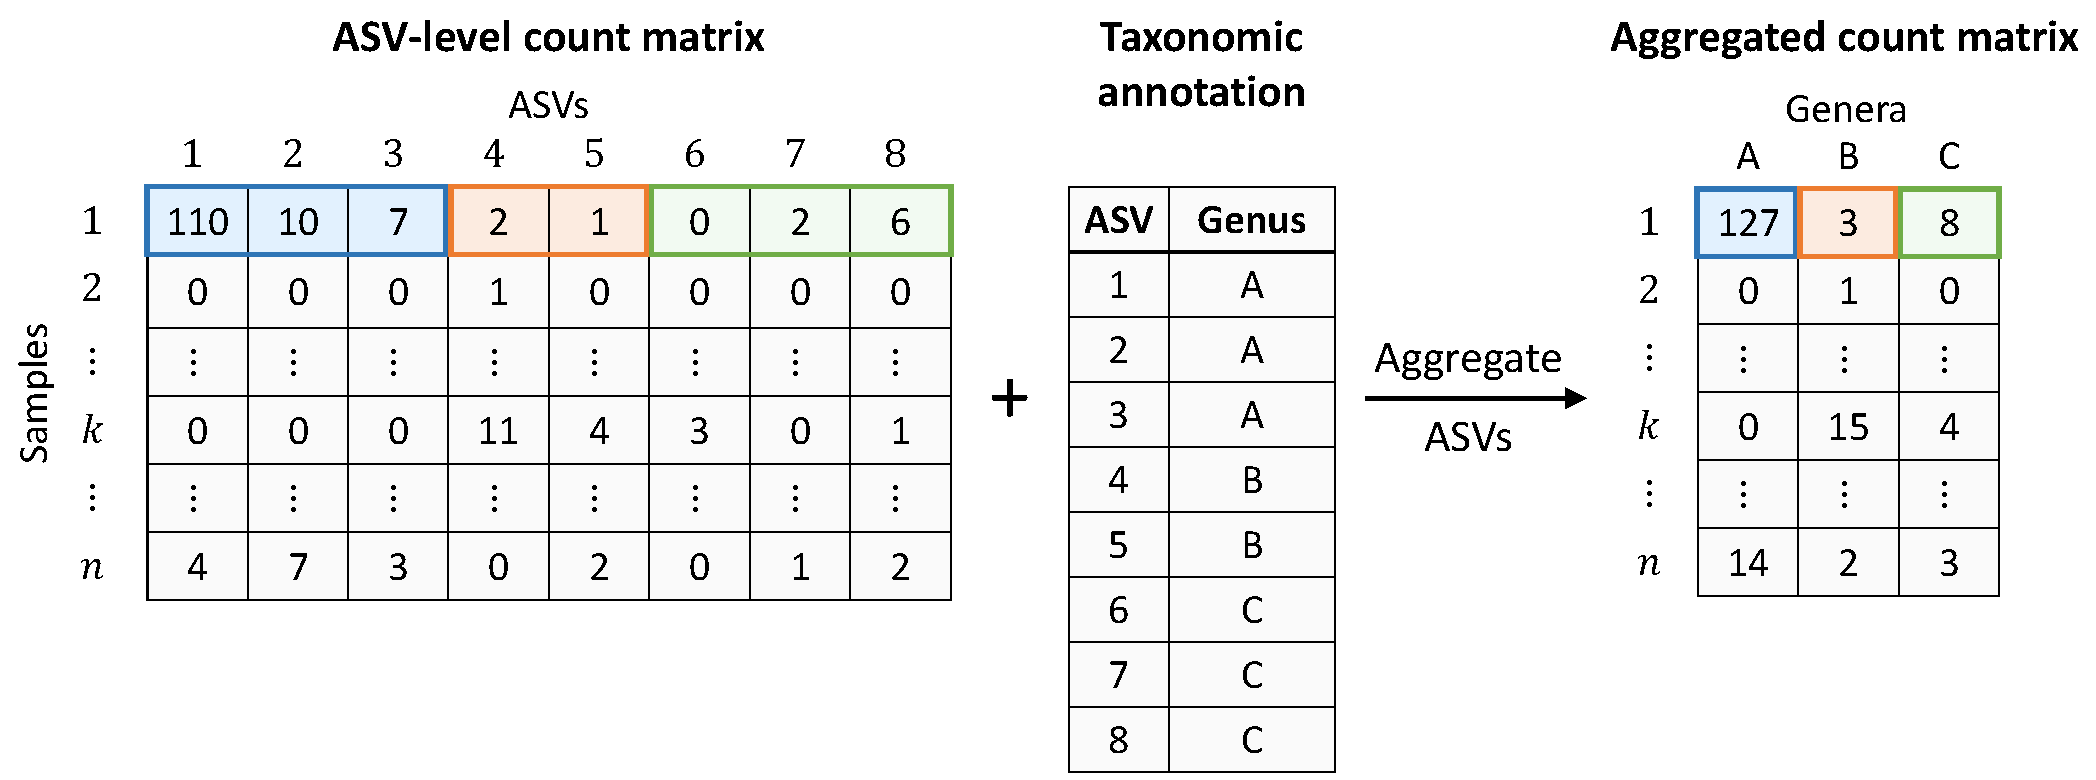
\includegraphics[width=\textwidth]{../ch02_microbiome_data/overview_figures/overview_aggregation.pdf}
\caption{\textbf{Overview of taxonomic aggregation.} The figure illustrates the aggregation of an ASV-level count matrix to genus level using the corresponding taxonomic annotation. The taxonomic table assigns each ASV to a genus, here denoted by A, B, and C. ASVs assigned to the same genus are combined by summing their counts within each sample, resulting in an aggregated count matrix with one column per genus.}
\label{fig:2micro:overview_aggregation}
\end{figure}

After primary bioinformatic processing, microbiome sequencing data are typically available as a feature table together with sample metadata and taxonomic annotations. In this thesis, we assume that read-level processing steps such as quality filtering, denoising, chimera removal, and feature inference have already been completed, for example using pipelines such as DADA2 \citep{callahan2016dada2}. The statistical analysis therefore starts from the resulting count matrix, and preprocessing refers to operations applied to this matrix before descriptive analysis, modeling, or hypothesis testing.

Before choosing the taxonomic resolution of the analysis, a minimal preliminary cleanup is usually applied to remove empty rows and columns from the selected data set. Samples with zero total counts cannot contribute to compositional analyses, and taxa with zero total counts in the retained samples contain no information for the corresponding analysis cohort. This preliminary removal of empty samples or taxa should be distinguished from abundance- or prevalence-based filtering, which is discussed in Section~\ref{sec:2micro:filtering} and is typically applied after the analysis feature space has been defined.

A common next preprocessing decision concerns the taxonomic resolution at which the microbiome is represented. Taxonomic aggregation combines lower-level features into higher-level taxonomic units according to their annotation. Figure~\ref{fig:2micro:overview_aggregation} illustrates this step for an ASV-level count matrix that is aggregated to genus level. The resulting matrix defines the feature space for the subsequent analyses.

Taxonomic aggregation is commonly performed by summing ASV- or OTU-level counts to genus, family, or phylum level. If $g(i)$ denotes the taxonomic group assigned to feature $i$, the aggregated count for group $h$ in sample $k$ is given by
\begin{equation}
x^{\mathrm{agg}}_{kh} = \sum_{i:g(i)=h} x_{ki}.
\label{eq:2micro:taxonomic_aggregation}
\end{equation}
The resulting count matrix has typically fewer columns than the original matrix and represents the microbiome at a coarser taxonomic resolution. In practical microbiome workflows in R, this operation is often implemented using the function \texttt{tax\_glom()} from the \texttt{phyloseq} package, which agglomerates features according to a selected taxonomic rank \citep{mcmurdie2013phyloseq}. The result depends on the available taxonomic annotation and on how unresolved assignments are handled. Such features may be retained as unclassified groups, aggregated at the lowest reliably assigned rank, or excluded; these choices should be reported because they affect the resulting feature space and downstream analyses.

Aggregation can reduce dimensionality and sparsity and may improve interpretability, especially when the original count matrix contains many rare ASVs or OTUs. It can also improve the numerical stability of downstream analyses, because higher-level taxa are often observed in more samples and with larger counts. At the same time, aggregation changes the biological and statistical object under investigation. A genus-level feature is not equivalent to a single organism, but represents the combined signal of all lower-level features assigned to that genus. Heterogeneous behavior within a taxonomic group may therefore be masked. For example, two ASVs assigned to the same genus may show opposite group-specific patterns, which can cancel after aggregation.

Taxonomic aggregation is therefore not merely a visualization decision, but determines the feature space and the hypotheses addressed by subsequent analyses. Testing at ASV level concerns differences in individual sequence variants between groups, whereas genus-level analysis concerns differences in the aggregated genus-level feature formed by the assigned variants. Similarly, community-level dissimilarities, feature-level test statistics, and estimated association networks may all change after aggregation, because summing lower-level features alters both marginal abundance patterns and pairwise relationships between the retained features. The chosen taxonomic level therefore defines the basis for subsequent filtering, normalization, zero handling, transformation, and inference.

However, aggregation to a single fixed rank is not equally suitable for all microbiome analyses. Some methods explicitly use the taxonomic hierarchy or combine information across multiple taxonomic levels. For example, tree-aggregated predictive modeling uses the phylogenetic or taxonomic tree to construct predictors at multiple aggregation levels and selects among them during model fitting \citep{bien2021treeaggregated}. In such settings, reducing the data to one preselected taxonomic rank may discard information that the method is designed to exploit. In the analyses presented in this thesis, however, the feature space is fixed before downstream preprocessing and inference. Unless stated otherwise, the application analyses are performed at genus level, so that subsequent filtering, normalization, zero handling, transformation, and statistical testing are applied to genus-level count matrices.


%%%%%%%%%%%%%%%%%%%%%%%%%%%%%%%%%%%%%
\section{Filtering of samples and taxa}
\label{sec:2micro:filtering}
%%%%%%%%%%%%%%%%%%%%%%%%%%%%%%%%%%%%%

\begin{figure}[H]
\centering
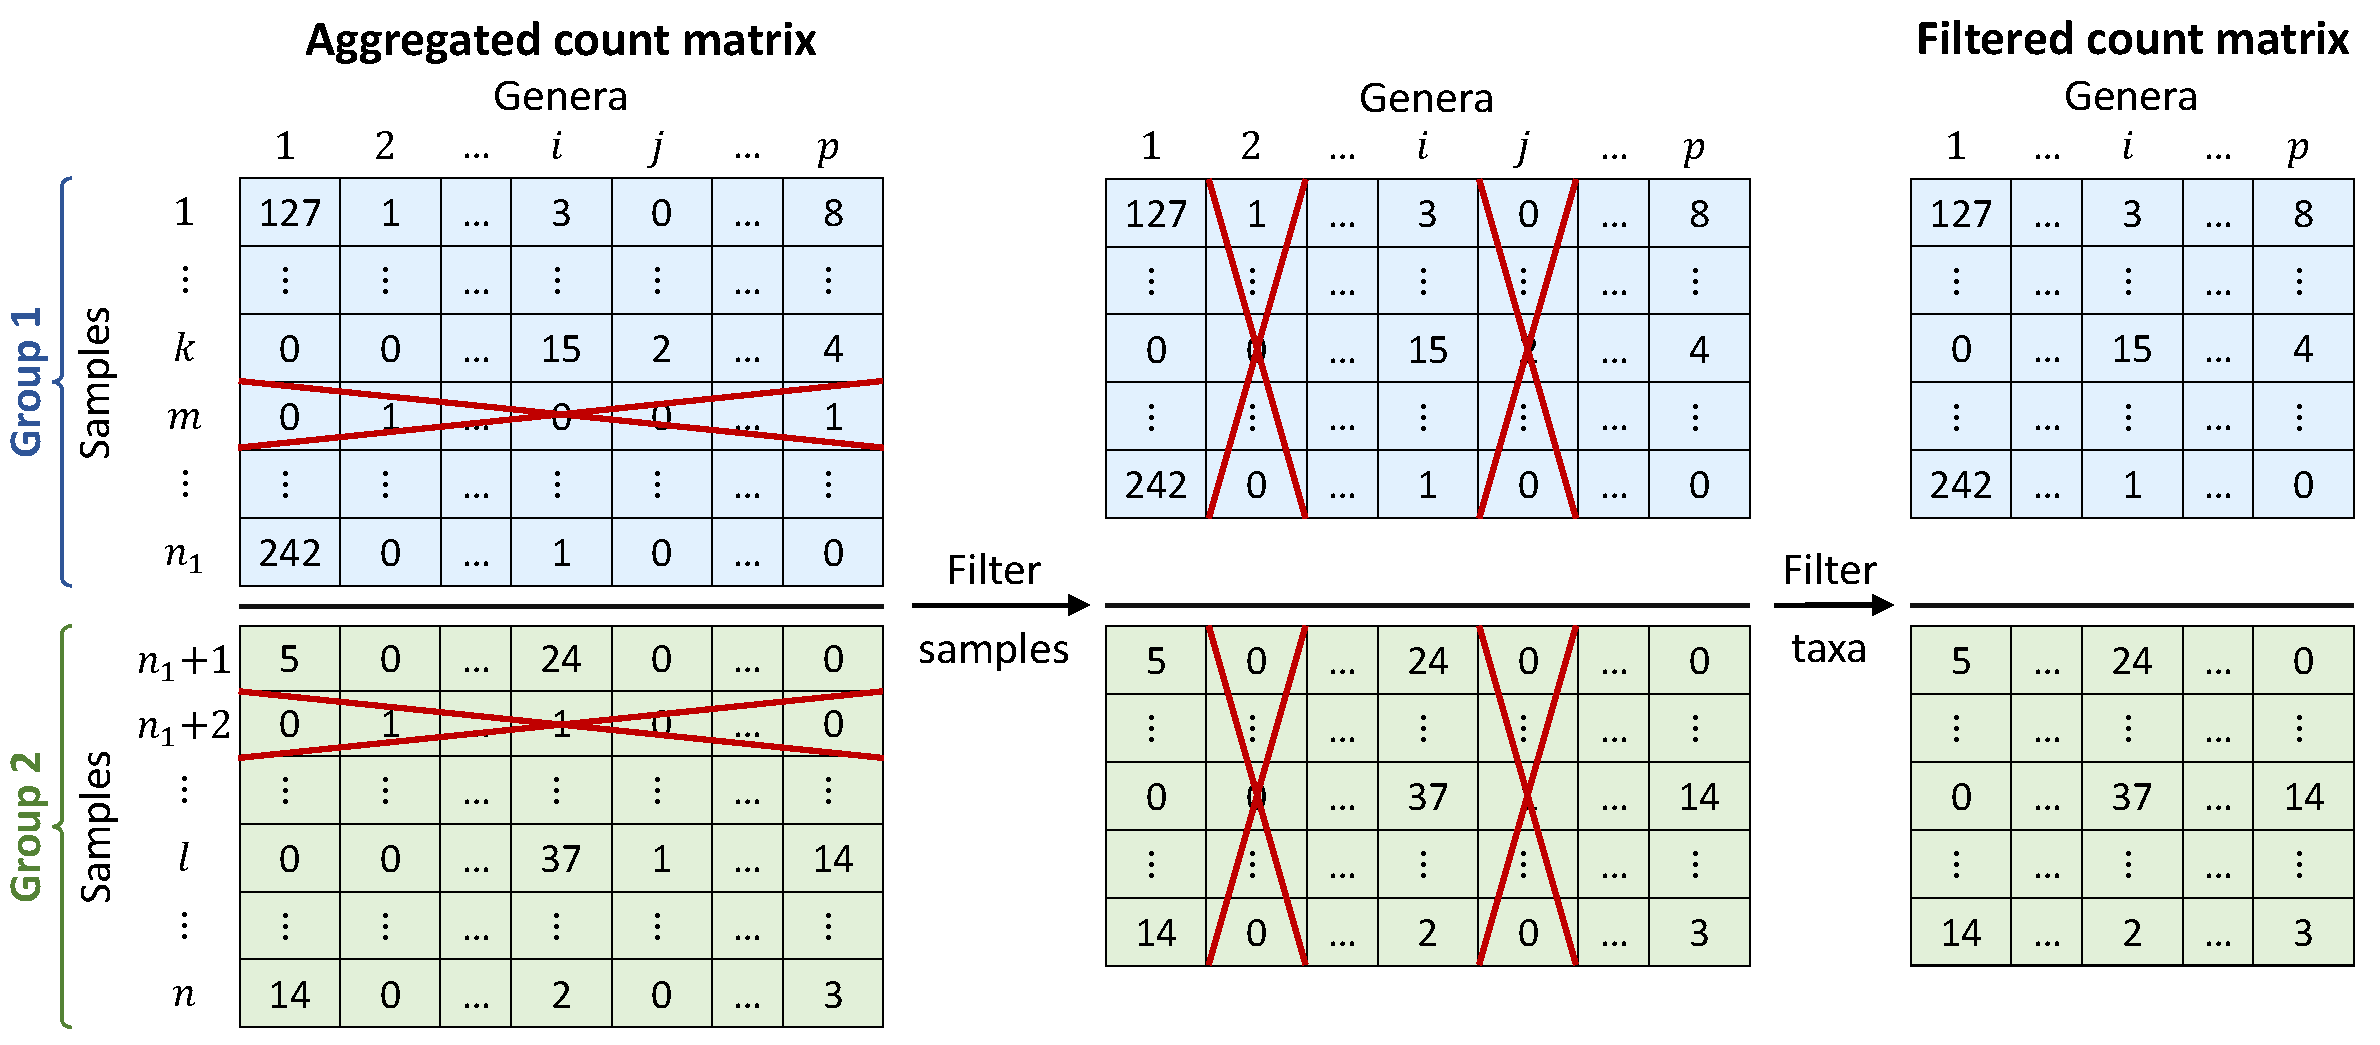
\includegraphics[width=\textwidth]{../ch02_microbiome_data/overview_figures/overview_filtering.pdf}
\caption{\textbf{Overview of sample and taxa filtering.} The figure illustrates filtering of an aggregated microbiome count matrix at genus level. Samples may be removed according to sample-level criteria, such as insufficient sequencing depth, missing metadata, or analysis eligibility. Genera may be removed according to feature-level criteria, such as low abundance, low prevalence, or insufficient variability. The two colored sample blocks represent two groups and are shown for consistency with later comparative analyses. Filtering criteria may be evaluated on the pooled data set or separately within groups, which can lead to different retained samples or genera.}
\label{fig:2micro:overview_filtering}
\end{figure}

After the taxonomic resolution of the analysis has been chosen, additional filtering may be applied to remove samples or taxa that provide little reliable information for the downstream analysis. Figure~\ref{fig:2micro:overview_filtering} illustrates this step for a count matrix represented at the selected taxonomic level. In contrast to the preliminary removal of empty rows and columns described in Section~\ref{sec:2micro:aggregation}, filtering in this section refers to analysis-level criteria such as sequencing depth, abundance, prevalence, and variability \citep{xia2024applied,weiss2017normalization}. Such filtering can improve numerical stability, reduce sparsity, and make the resulting feature space more interpretable. At the same time, it changes the data object under study and may influence downstream inference. Filtering should therefore be viewed not as a purely technical cleaning step, but as an analysis decision that needs to be reported and justified.

From this point onward, the overview figures display two sample groups, reflecting the comparative focus of later chapters. The grouping is included for visual consistency and does not imply that preprocessing is necessarily group-specific. However, in group comparison settings, filtering criteria may be evaluated either on the pooled data set or separately within groups. For example, a pooled prevalence filter asks whether a taxon is observed sufficiently often across the complete analysis cohort, whereas a group-wise filter may require that the taxon is observed in each group. These choices can lead to different retained feature sets and therefore affect the precise target of inference. For comparative analyses, pooled filtering is often preferable when the aim is to define a common feature space independently of group membership. Group-wise filtering may be appropriate in specific settings, but it can exclude taxa that are prevalent in only one group and may therefore remove part of the very signal under investigation.

In practice, filtering is performed at two levels. Sample filtering removes entire samples, most commonly because their library size is considered too small for reliable analysis or because relevant metadata are unavailable. Taxa filtering removes features that are too rare, too sparse, or insufficiently variable to support stable estimation for the intended downstream analysis. Both levels are discussed in the following.

%====================================
\subsection{Sample filtering}
\label{sec:2micro:filtering:samples}
%====================================

Sample filtering removes entire samples based on quality, metadata availability, or sequencing depth criteria. A common approach is to exclude samples with low library size. In practice, thresholds vary substantially across studies. For instance, samples with fewer than 500 reads \citep{carcy2024metaibs}, 2,150 reads \citep{kirjavainen2019farmlike}, 4,000 reads \citep{kennedy2014evaluating}, or 10,000 reads \citep{parada2016every} have been excluded in different analyses.
No universally valid threshold exists, because the information contained in a given library size depends on community complexity, the taxonomic resolution, the sequencing protocol, and the downstream analysis.
The rationale is that low-depth samples provide limited information, especially on low-abundance taxa, and are more susceptible to sampling zeros \citep{martin2011dealing}. In addition, contaminant DNA may account for a larger relative proportion of reads when the true microbial biomass or sequencing yield is low \citep{salter2014reagent}.

%====================================
\subsection{Taxa filtering}
\label{sec:2micro:filtering:taxa}
%====================================

Taxa filtering removes features, such as ASVs, OTUs, or genera, based on abundance, prevalence, or variability criteria. 
Since the present section follows taxonomic aggregation, these criteria are understood to apply to the feature space used in the analysis. Thus, for a genus-level analysis, prevalence or abundance filtering is applied to genera rather than to the lower-level ASVs or OTUs from which they were formed. This distinction is important because filtering before aggregation and filtering after aggregation generally lead to different data objects.

Several classes of filtering rules are commonly used in the literature:

\noindent\textbf{Total abundance filtering:} Retain taxa whose total number of reads across all samples exceeds a predefined threshold, for example 50 reads \citep{kirjavainen2019farmlike,roggenbuck2014microbiome}.

\noindent\textbf{Relative abundance filtering:} Retain taxa whose total abundance exceeds a specified proportion of the overall read count, for example 0.05\% \citep{bokulich2013qualityfiltering}.

\noindent\textbf{Prevalence filtering:} Retain taxa observed in at least a specified number or proportion of samples, for example 10\% \citep{carcy2024metaibs}.

\noindent\textbf{Variance-based filtering:} Retain taxa whose empirical variance across samples exceeds a predefined threshold, thereby excluding invariant or near-invariant features that cannot contribute to exploratory discrimination or association analyses \citep{borman2024orchestrating}. For confirmatory feature-level testing, variance filtering should be used cautiously because the empirical variance may itself reflect group differences.

The choice of taxa filtering criterion should be aligned with the downstream analysis. For exploratory summaries and visualizations, stricter filtering may improve interpretability by focusing on commonly observed taxa. For feature-level hypothesis testing, filtering can reduce the multiple testing burden but also restricts the set of hypotheses being tested. For network analysis, removing extremely rare taxa may improve the stability of association estimates and also the interpretability of the network plot, but excessive filtering may also remove biologically relevant low-prevalence organisms. Consequently, taxa filtering should be specified before testing whenever possible, preferably using criteria that do not depend on the observed group difference, and interpreted as part of the definition of the analysis feature set.

%%%%%%%%%%%%%%%%%%%%%%%%%%%%%%%%%%%%%
\section{Normalization and library-size adjustment}
\label{sec:2micro:normalization}
%%%%%%%%%%%%%%%%%%%%%%%%%%%%%%%%%%%%%

\begin{figure}[H]
\centering
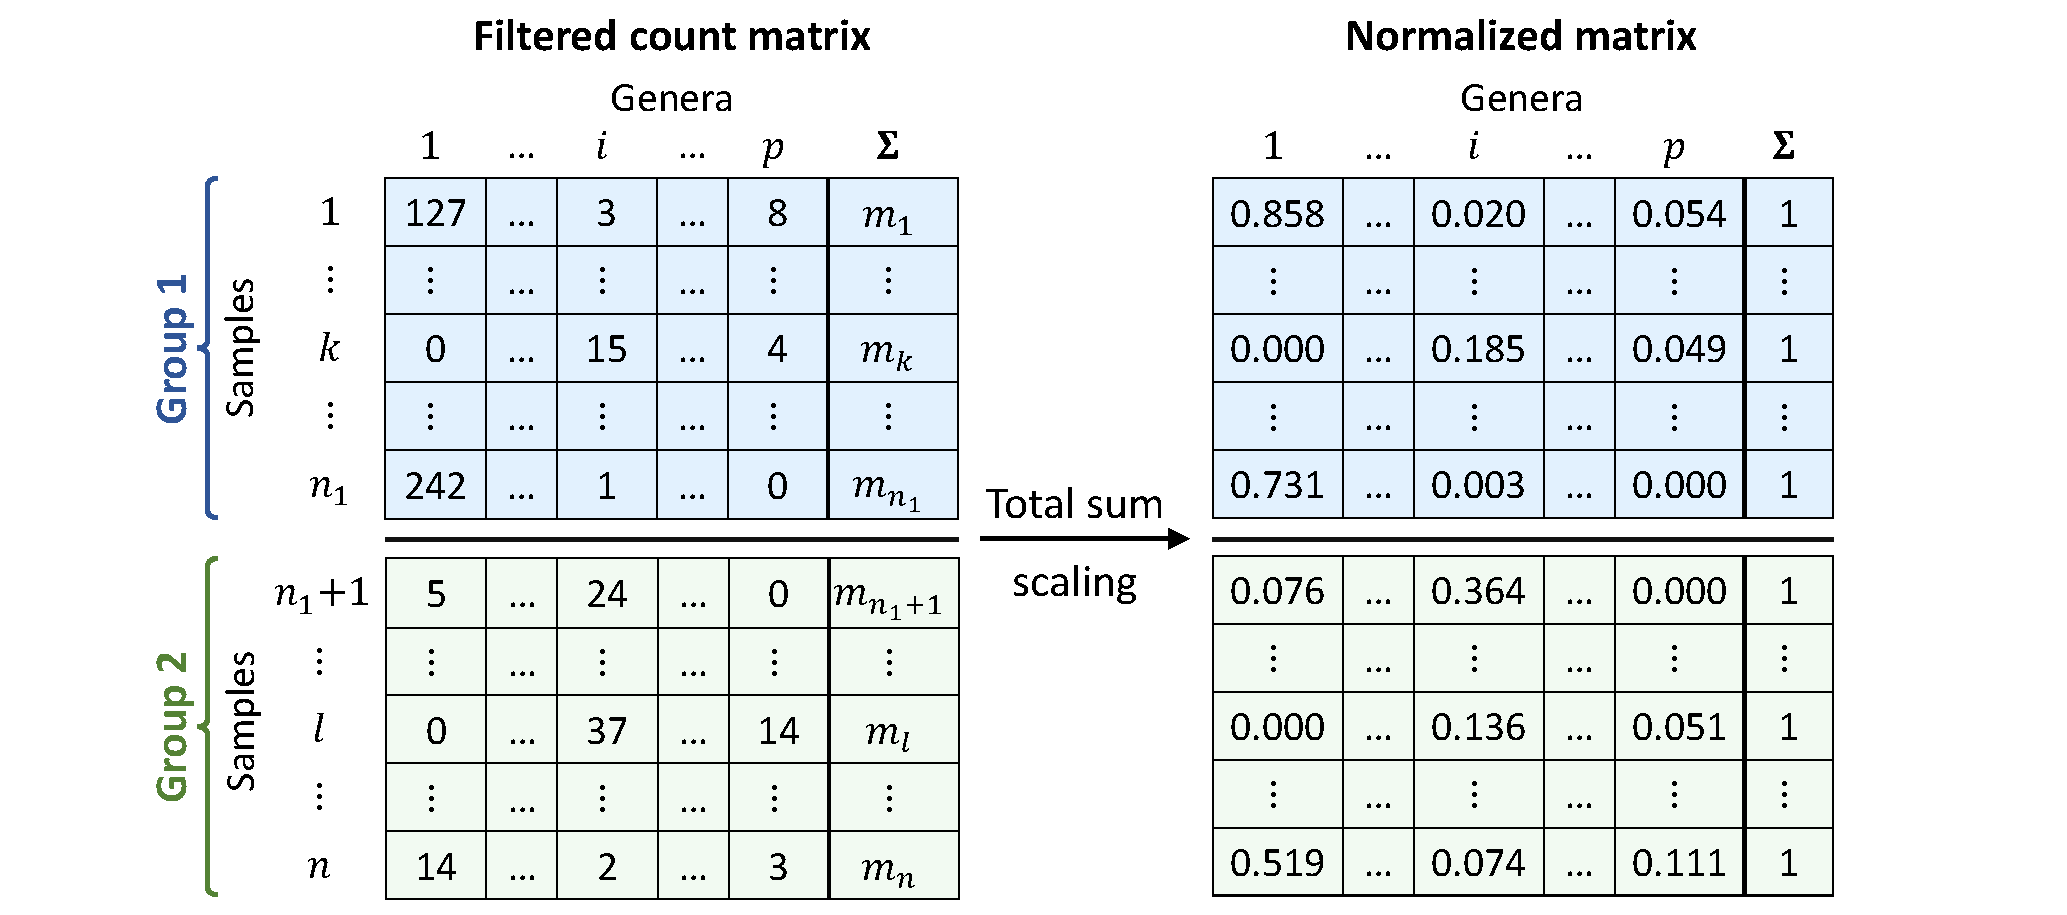
\includegraphics[width=\textwidth]{../ch02_microbiome_data/overview_figures/overview_normalization.pdf}
\caption{\textbf{Overview of normalization by total sum scaling.} The figure illustrates library-size adjustment of a filtered genus-level count matrix by total sum scaling. For each sample, counts are divided by the corresponding library size, shown in the column $\Sigma$ of the count matrix. The resulting normalized matrix contains relative abundances, here rounded to three decimal places, and each row sums to one before rounding. The two colored sample blocks represent two groups and are shown for consistency with later comparative analyses. The normalization step itself is applied sample-wise and is not group-specific.}
\label{fig:2micro:overview_normalization}
\end{figure}

After filtering and taxonomic aggregation, microbiome count matrices still contain samples with heterogeneous library sizes. Since the total number of reads differs between samples, raw counts are not directly comparable across samples: a taxon with the same relative contribution to two microbial communities will, on average, yield more reads in the sample with larger library size. Normalization aims to reduce artifactual variation induced by uneven sequencing depth, thereby making measurements from different samples more comparable \citep{weiss2017normalization}. It does not, however, generally remove other sources of technical variation, such as batch effects or taxon-specific amplification bias. In the narrower sense used in this chapter, normalization refers to preprocessing steps that adjust for heterogeneous library sizes or bring samples to a common compositional scale, without changing the coordinate system in which the data are represented.

Figure~\ref{fig:2micro:overview_normalization} illustrates this idea for total sum scaling, the normalization step used in the CLR-based analyses of this thesis. Starting from the filtered genus-level count matrix, each row is divided by its corresponding library size. The resulting normalized matrix contains relative abundances, and each sample sums to one. Thus, total sum scaling removes differences in the total count scale while preserving the within-sample ratios among non-zero counts.


This distinction between normalization and transformation is important because both terms are sometimes used interchangeably in the microbiome literature. In this thesis, transformations are treated separately in Section~\ref{sec:2micro:transformation}: they map the data into a new representation, for example by stabilizing variance or by expressing compositions in log-ratio coordinates. Normalization, by contrast, acts before such transformations and addresses the fact that samples may have been sequenced to different depths.

The ordering of preprocessing steps matters in particular for analyses based on log-ratio transformations. Since log-ratio transformations require strictly positive components, zero replacement is needed before applying them. However, if replacement values are defined on the raw count scale, the same numerical replacement value has different relative weight in samples with different library sizes. For this reason, the CLR-based analyses in this thesis first bring samples to a common compositional scale by total sum scaling, then perform zero replacement, and finally apply the CLR transformation. The present section introduces normalization methods for library-size adjustment, while zero handling and transformations are discussed in the following sections.

%====================================
\subsection{Scaling-based library size adjustment}
\label{sec:2micro:norm:scaling}
%====================================

A common strategy for addressing heterogeneous library sizes consists of rescaling counts by sample-specific factors. 
In general form, scaling replaces the original counts $x_{ki}$ by
\begin{equation}
\tilde{x}_{ki} = \frac{x_{ki}}{s_k}, \qquad k=1,\dots,n,\;i=1,\dots,p,
\end{equation}
where $s_k>0$ is a sample-specific scaling factor. 
The choice of $s_k$ determines the normalization method.

%------------------------------------
\subsubsection*{Total sum scaling (TSS)}
%------------------------------------

The simplest scaling-based approach uses the observed library size $m_k=\sum_{i=1}^p x_{ki}$ as the sample-specific scaling factor. This leads to \emph{total sum scaling} (TSS), where each count is divided by the total number of reads in the corresponding sample:
\begin{equation}
\tilde{x}^{\mathrm{TSS}}_{ki} = \frac{x_{ki}}{m_k}.
\end{equation}
The resulting values are relative abundances and each normalized sample satisfies $\sum_{i=1}^p \tilde{x}^{\mathrm{TSS}}_{ki}=1$. TSS therefore places all samples on a common total-count scale and removes variation due solely to differences in the observed library size.

However, TSS does not remove the compositional dependence induced by closure. Moreover, it does not account for the fact that detection probabilities depend on sequencing depth. Rare taxa that are unobserved in shallow samples may appear at low but non-zero relative abundances in deeper samples, potentially distorting prevalence estimates and correlation patterns \citep{weiss2017normalization}. In addition, because all components are scaled by the total library size, a few highly abundant taxa can strongly influence the normalized values of all other taxa. Several alternative scaling procedures therefore replace the total library size $m_k$ by more robust estimates of the sample-specific scaling factor $s_k$, typically under structural assumptions about the majority of taxa being unchanged or about the influence of highly abundant features.

%------------------------------------
\subsubsection*{Cumulative sum scaling (CSS)}
%------------------------------------

Cumulative sum scaling (CSS) replaces the total library size $m_k$ by a partial sum of the count distribution. More precisely, the scaling factor $s_k$ is defined as the cumulative sum of counts up to a data-driven percentile, excluding the largest counts from the normalization factor \citep{paulson2013differential,badri2020shrinkage}. The motivation is that highly abundant taxa can dominate the total library size and thereby influence the normalized values of all remaining taxa. By using only a lower part of the count distribution, CSS aims to reduce this sensitivity while still adjusting for differences in sequencing depth.

%------------------------------------
\subsubsection*{Common sum scaling (COM)}
%------------------------------------

Common sum scaling (COM) rescales all samples to a common library size, usually chosen as the smallest observed library size $m_{\min}=\min_k m_k$. In the scaling formulation, this corresponds to using
\begin{equation}
s_k = \frac{m_k}{m_{\min}},
\end{equation}
so that the rescaled counts satisfy $\sum_{i=1}^p \tilde{x}_{ki}=m_{\min}$ for each sample $k$ \citep{badri2020shrinkage}. Unlike rarefaction (cf. Section~\ref{sec:2micro:norm:rarefaction}), which also aims to equalize library sizes, COM achieves this by deterministic rescaling rather than by random subsampling.

%------------------------------------
\subsubsection*{Relative log expression (RLE)}
%------------------------------------

Size-factor methods originally developed for RNA-seq data have also been adapted to microbiome count data. These approaches estimate $s_k$ under the assumption that most features do not exhibit systematic changes across the samples or conditions under study, so that a typical multiplicative difference can be interpreted as a technical size factor rather than as a global biological shift. The relative log expression (RLE) method implemented in the \texttt{DESeq2} \textsf{R} package \citep{love2014moderated} computes, for each sample, the median ratio of counts to a pseudo-reference sample defined by the geometric mean across samples \citep{badri2020shrinkage}. The resulting size factor represents the typical multiplicative deviation of that sample from the reference.

%------------------------------------
\subsubsection*{Trimmed mean of M-values (TMM)}
%------------------------------------

The trimmed mean of M-values (TMM) normalization implemented in \texttt{edgeR} \citep{robinson2010edger,chen2025edger} estimates scaling factors based on log fold changes relative to a reference sample. To reduce the influence of extreme observations, the calculation trims features with very large log fold changes or expression levels before computing the normalization factor. This makes TMM less sensitive to highly abundant or strongly differential features than simple total-sum based scaling \citep{baruzzo2022beware}.

%------------------------------------
\subsubsection*{Geometric mean of pairwise ratios (GMPR)}
%------------------------------------

The geometric mean of pairwise ratios (GMPR) method was proposed specifically for sparse sequencing data with many zero counts \citep{chen2018gmpr}. Instead of relying on a pseudo-reference based on feature-wise geometric means, which can be problematic when many features contain zeros, GMPR estimates sample-specific size factors from median pairwise ratios between samples. This construction makes the method more robust in sparse microbiome count matrices, where many taxa are absent or unobserved in a large fraction of samples. 

The assumptions underlying the RLE and TMM approaches were originally developed for gene-expression data and may be difficult to justify in microbiome studies when a substantial proportion of taxa changes jointly between groups or when compositional effects dominate the observed counts.

%====================================
\subsection{Rarefaction}
\label{sec:2micro:norm:rarefaction}
%====================================

The scaling-based methods discussed above adjust for heterogeneous library sizes by multiplying all counts in a sample by a sample-specific factor. Rarefaction follows a different principle. Instead of rescaling the observed counts, it equalizes library sizes by randomly subsampling reads from each sample to a common target depth $m_{\mathrm{rare}}$, usually without replacement \citep{mcmurdie2014waste}. The target depth is often chosen as the smallest observed library size $m_{\min}=\min_k m_k$ or as a larger quantile of the library-size distribution. In the latter case, samples with library sizes below the chosen target must be excluded from the rarefied data set. Conditional on the observed count vector $\mathbf{x}_k=(x_{k1},\ldots,x_{kp})^\top$, the rarefied count vector can be viewed as a random draw from the observed reads and satisfies
\begin{equation}
\sum_{i=1}^p \tilde{x}^{\mathrm{rare}}_{ki} = m_{\mathrm{rare}}.
\end{equation}
More explicitly, this subsampling step can be described by a multivariate hypergeometric distribution,
\begin{equation}
\tilde{\mathbf{x}}^{\mathrm{rare}}_k \sim \operatorname{MultivariateHypergeometric}\left(m_{\mathrm{rare}},x_{k1},\ldots,x_{kp}\right).
\end{equation}

Rarefaction directly enforces equal library sizes and is therefore particularly intuitive for analyses based on ecological dissimilarities or observed diversity measures, where unequal sampling effort can otherwise dominate comparisons between samples. At the same time, rarefaction modifies the observed count matrix in a fundamentally different way than deterministic rescaling: it discards reads from samples with library size larger than $m_{\mathrm{rare}}$, introduces additional sampling variability, and may turn originally non-zero low counts into zeros.

For this reason, rarefaction has been one of the most controversial preprocessing steps in microbiome data analysis. \citet{mcmurdie2014waste} argued that rarefying is statistically inadmissible because it discards observed counts, reduces power, and performs unfavorably compared with model-based approaches in differential abundance settings. In contrast, \citet{schloss2023waste} revisited this conclusion and argued that the original comparison was affected by simulation and analysis choices that made rarefaction appear worse than it is. More recently, \citet{schloss2026rarefaction} further argued, based on simulations and re-analyses of case studies, that rarefaction can control uneven sequencing effort more effectively than robust Aitchison PCA and several other compositional or normalization-based approaches in distance-based analyses of amplicon data.

These apparently conflicting conclusions are less contradictory when the downstream analysis target is made explicit. Rarefaction is mainly relevant when the objective is to compare community-level summaries, such as alpha diversity, beta diversity, ordination, or PERMANOVA-type analyses, under heterogeneous library sizes. In such settings, equalizing the number of reads can reduce the extent to which distances or diversity estimates reflect sampling effort rather than biological variation. For feature-level differential abundance testing or association network estimation, however, rarefaction is generally not a universal solution. Several differential abundance methods model raw counts and incorporate their own adjustment for library size or sampling depth, while compositionally-aware network methods often rely on log-ratio, proportionality, or sparse graphical-model approaches. Rarefying before such methods may unnecessarily increase sparsity and remove information that the model is designed to use. Thus, rarefaction should not be understood as a generally optimal normalization strategy, but as a context-dependent tool whose usefulness depends on the inferential target and the assumptions of the downstream method.

%%%%%%%%%%%%%%%%%%%%%%%%%%%%%%%%%%%%%
\section{Handling zero counts}
\label{sec:2micro:zeros}
%%%%%%%%%%%%%%%%%%%%%%%%%%%%%%%%%%%%%

\begin{figure}[H]
\centering
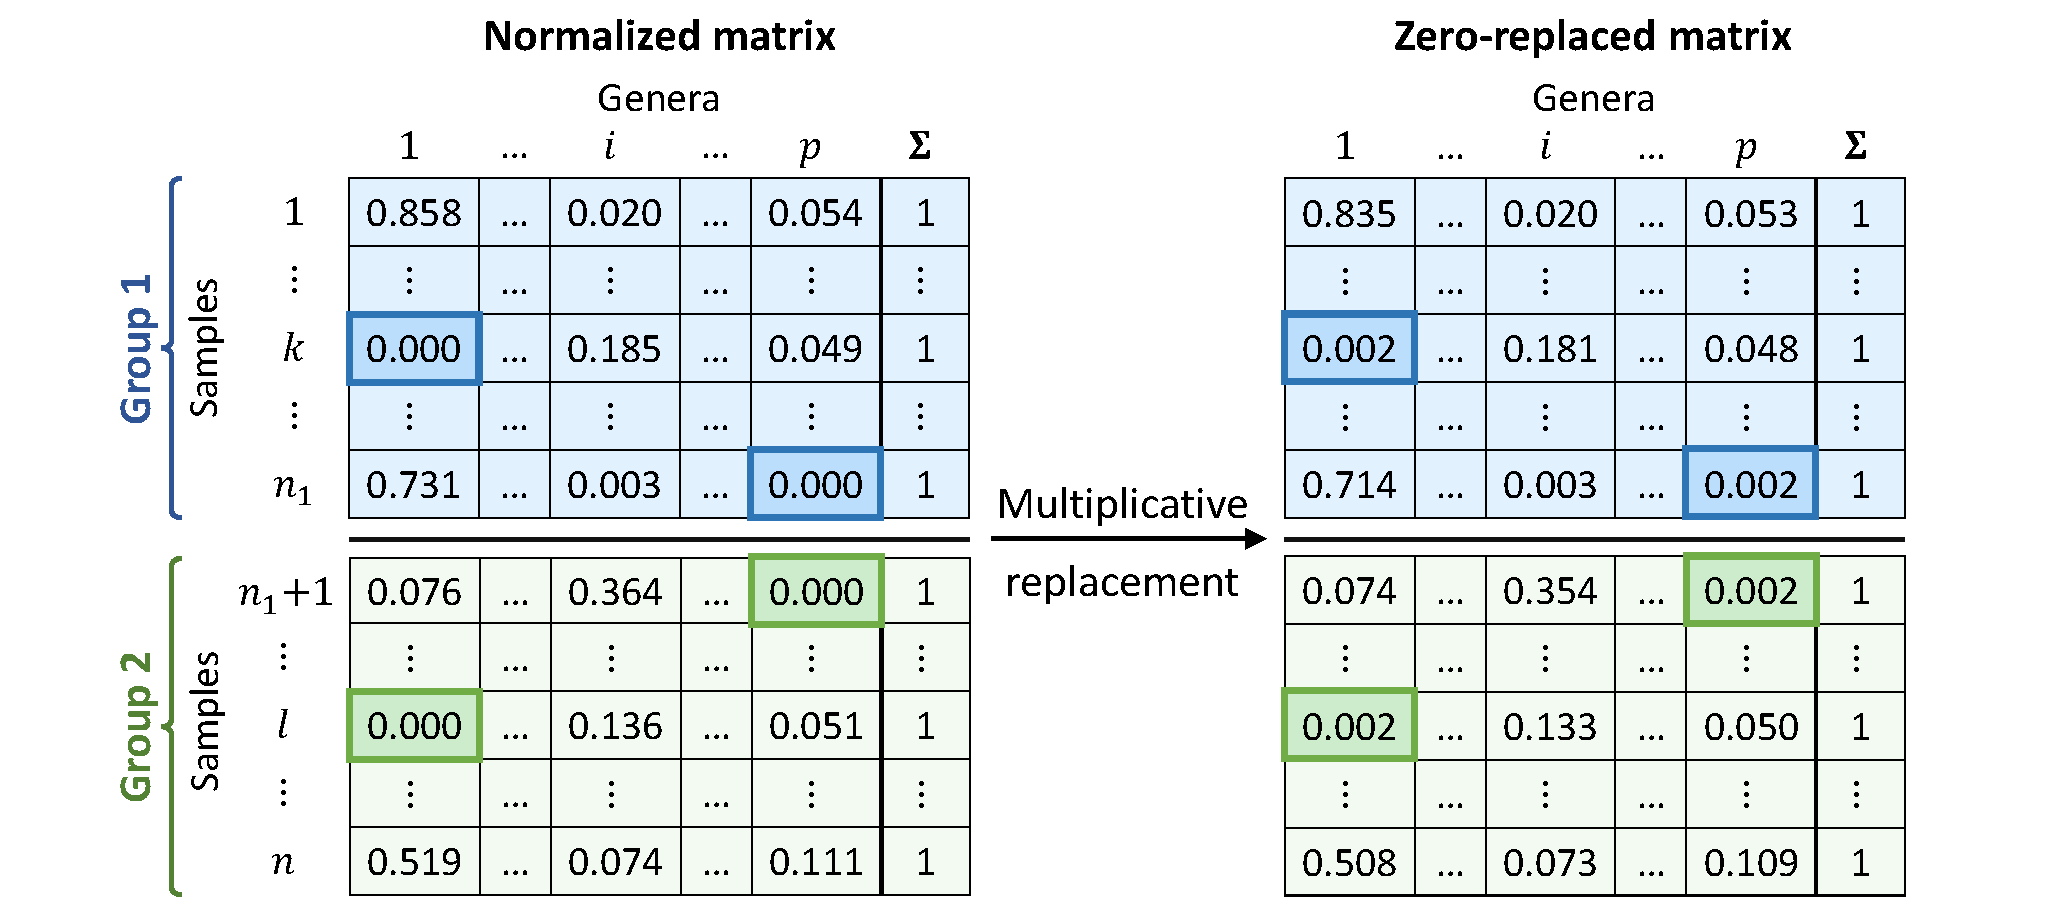
\includegraphics[width=\textwidth]{../ch02_microbiome_data/overview_figures/overview_zero_replacement.pdf}
\caption{\textbf{Overview of zero replacement by multiplicative replacement.} The figure illustrates zero replacement for a normalized genus-level matrix after total sum scaling. Zero entries are replaced by a small positive value $\delta$, while the non-zero entries in the same sample are adjusted multiplicatively so that the sample remains on the same compositional scale. In the example shown, the detection limit $DL$ is defined as the minimum non-zero matrix entry, and the replacement value is chosen as $\delta = 0.65 \cdot DL$, corresponding to the default setting in \texttt{multRepl()}. Matrix entries are rounded to three decimal places, so that the replacement value appears as $0.002$. The two colored sample blocks represent two groups and are shown for consistency with later comparative analyses. The zero-replacement step itself is applied sample-wise and is not group-specific.}
\label{fig:2micro:overview_zeros}
\end{figure}

Even after filtering and library-size adjustment, microbiome data usually remain sparse and contain many zero entries. These zeros are not merely inconvenient numerical values, but may reflect biological absence, limited sequencing depth, detection limits, or other technical aspects of the measurement process. Their interpretation is therefore ambiguous: the same observed value $x_{ki}=0$ may indicate that taxon $i$ is truly absent from sample $k$, or that it was present but not observed by the sequencing process.

This ambiguity matters because many statistical models interpret a zero count according to an implicit data-generating mechanism, for example as an observed count outcome or as evidence of absence. For count-based models, this may affect assumptions about the data-generating process and dispersion structure. For compositional methods, the problem is even more direct: log-ratio transformations require strictly positive components and are therefore undefined in the presence of zeros. Zero handling is thus not only a computational prerequisite for some methods, but also a modeling decision about how unobserved or undetected taxa should enter the analysis.

\newpage
In the preprocessing order used in this thesis for CLR-based analyses (cf. Section~\ref{sec:2micro:preprocessing_choices_thesis}), zero replacement is applied after bringing samples to a common compositional scale by total sum scaling. This order is important because replacement values defined on the raw count scale would have different relative weight in samples with different library sizes. Applying zero replacement on the relative abundance scale instead makes the imputed values comparable across samples in compositional terms. At the same time, the general principles discussed below apply more broadly to compositional vectors with arbitrary constant sum. Figure~\ref{fig:2micro:overview_zeros} illustrates this step for multiplicative replacement, which is the default zero-handling approach used later for CLR-based analyses.

In the following, we first distinguish the main types of zeros discussed in compositional data analysis and microbiome methodology. We then summarize common replacement and imputation strategies and discuss their implications for downstream analyses.

%====================================
\subsection{Types of zeros}
\label{sec:2micro:zeros:types}
%====================================

Several classifications of zeros have been proposed in the compositional data analysis (CoDA) literature and in microbiome methodology.

A common distinction proposed by \citet{martin2011dealing} differentiates between:

\begin{itemize}
    \item \textbf{Essential / structural zeros:} The taxon is assumed to be truly absent from the sample. Under this interpretation, replacing the zero by a small positive value would be inappropriate.
    
    \item \textbf{Rounded zeros:} The taxon is present but its abundance lies below a detection limit or is rounded to zero due to measurement precision.

    \item \textbf{Count / sampling zeros:} The taxon is present in the environment but not observed due to limited sequencing depth.
\end{itemize}

For next-generation sequencing data, \citet{quinn2019field} emphasize that many observed zeros may arise through finite sampling, since increasing sequencing depth can reveal additional low-abundance taxa.
Similarly, \citet{paulson2013differential} report a strong association between sequencing depth and the number of detected taxa, which is consistent with at least some zeros reflecting undersampling rather than true absence.

\citet{kaul2017analysis} introduce an alternative classification distinguishing structural zeros, sampling zeros, and \emph{outlier zeros}, where the latter arise from extraneous technical effects rather than detection limits. 

Importantly, the nature of a zero is typically not identifiable from the observed count matrix alone. The classification therefore depends on substantive knowledge and modeling assumptions.

%====================================
\subsection{Replacement and imputation strategies}
\label{sec:2micro:zeros:replacement}
%====================================

Because log-ratio transformations require strictly positive values, zero handling often involves either replacing zeros by small positive values or imputing them using a statistical model. 
These approaches differ in how strongly they perturb the relative structure of the data and in the extent to which they preserve compositional properties such as scale invariance and subcompositional coherence. In the following, it is useful to distinguish between strategies that add an offset to all components, strategies that replace only zero components, and imputation methods that use multivariate structure across samples and taxa.

\noindent\textbf{Global offset addition.}
A simple strategy often used in microbiome analysis is to add a constant, for example $1$, to all counts before applying a logarithmic transformation \citep{mcmurdie2013phyloseq,weiss2017normalization}. This strategy is computationally convenient because it makes all components positive. However, it modifies all components, including those that were originally non-zero. Consequently, ratios among observed components are changed. For example, for two positive components $x_i>0$ and $x_j>0$, adding a constant $\delta>0$ changes the ratio from
$x_i/x_j$ to $(x_i+\delta)/(x_j+\delta)$.
These two ratios are generally not equal. Thus, global offset addition does not only resolve zeros, but also perturbs relative information among taxa that were observed. As illustrated in Table~\ref{tab:zero_replacement}, this alters ratios among originally non-zero components and therefore changes the relative structure of any subcomposition containing them.

\noindent\textbf{Zero-only replacement.}
A simple strategy is to replace only entries equal to zero by a small positive value while leaving the non-zero components unchanged. This preserves ratios among originally non-zero components, because the positive entries themselves are not altered relative to one another. However, if the data are treated as compositions, the components are constrained to a fixed total, either on the count scale or after closure to unit sum. The positive mass assigned to zeros must therefore be accounted for. Without an appropriate adjustment of the positive components, the total sum of the modified composition increases, and the resulting vector no longer lies in the same simplex as the original composition. Thus, zero-only replacement is useful for illustrating the principle of preserving observed ratios, but a coherent replacement of a composition usually requires an additional rescaling step. Multiplicative replacement implements this idea by assigning small positive values to zeros and reducing the originally non-zero components proportionally.

\noindent\textbf{Multiplicative replacement.}
To preserve ratios among non-zero components while maintaining the compositional structure, \citet{martin-fernandez2003dealing} proposed multiplicative replacement. In contrast to global offset addition, multiplicative replacement does not add a constant to all components. Instead, zero components are replaced by small positive values and the originally non-zero components are adjusted proportionally so that the constant-sum constraint is preserved.
Although the notation below is written for a generic non-negative composition, in the default CLR-based pipeline of this thesis the vector entering multiplicative replacement is the relative abundance vector obtained after total sum scaling.

For sample $\mathbf{x}_k=(x_{k1},\ldots,x_{kp})^\top$ with sample total
\begin{equation}
C_k=\sum_{i=1}^p x_{ki},
\label{eq:2micro:sample_total_multiplicative_replacement}
\end{equation}
let $Z_k=\{i:x_{ki}=0\}$ denote the set of zero components. Following the formulation of \citet{martin-fernandez2003dealing}, the replacement can be written as
\begin{equation}
x_{ki}^\ast =
\begin{cases}
\delta_i, & x_{ki}=0,\\
\left(1-\frac{\sum_{j\in Z_k}\delta_j}{C_k}\right)x_{ki}, & x_{ki}>0,
\end{cases}
\label{eq:2micro:multiplicative_replacement_general}
\end{equation}
where $\delta_i>0$ is the imputed value for component $i$. The proportional factor applied to all non-zero components ensures that the sample total remains unchanged:
\begin{equation}
\sum_{i=1}^p x_{ki}^\ast = C_k.
\label{eq:2micro:multiplicative_replacement_total}
\end{equation}
This formulation allows component-specific replacement values, which is useful when detection limits differ between taxa or features.

For the replacement to be well defined, the total imputed mass must satisfy
\begin{equation}
	\sum_{j\in Z_k}\delta_j < C_k,
\end{equation}
so that the multiplicative adjustment factor for the originally non-zero components remains positive.

Since all originally non-zero components within sample $k$ are multiplied by the same factor, ratios among them are preserved. If $x_{ki}>0$ and $x_{kj}>0$, then
\begin{equation}
\frac{x_{ki}^\ast}{x_{kj}^\ast}
=
\frac{\left(1-\frac{\sum_{\ell\in Z_k}\delta_\ell}{C_k}\right)x_{ki}}
{\left(1-\frac{\sum_{\ell\in Z_k}\delta_\ell}{C_k}\right)x_{kj}}
=
\frac{x_{ki}}{x_{kj}}.
\label{eq:2micro:multiplicative_replacement_ratio}
\end{equation}
This ratio preservation is a key reason why multiplicative replacement is commonly used before log-ratio transformations. It differs from additive modifications of non-zero components, which can alter ratios among parts that were originally observed. Table~\ref{tab:zero_replacement} illustrates these differences for a simple three-part composition.

In practice, nonparametric multiplicative replacement for rounded or left-censored zeros is implemented, for example, in the function \texttt{multRepl()} of the \texttt{zCompositions} package \citep{palarea-albaladejo2015zcompositions}. This function requires a detection limit for each component and, by default, replaces a zero by a fraction of this limit. In sequencing data, however, detection limits are not always explicitly defined in the same way as in classical censored compositional data. Therefore, replacement values should be chosen in accordance with the scale and preprocessing context of the analysis.

\begin{table}[!htb]
\centering
\caption{Illustration of ratio preservation and subcompositional coherence for the composition $\mathbf{x}=(x_1,x_2,x_3)^\top$ with subcomposition $\operatorname{sub}(\mathbf{x})=(x_2,x_3)^\top$. The table compares global offset addition, zero-only replacement, and multiplicative replacement. The replacement value in each case is $\delta = 0.1$. Global offset addition changes the ratio $x_2/x_3$ and alters the relative structure of the subcomposition. In contrast, zero-only replacement and multiplicative replacement preserve the ratio among originally non-zero components. Multiplicative replacement additionally preserves the compositional total by proportionally adjusting the non-zero components.}
\label{tab:zero_replacement}
\small
\setlength{\tabcolsep}{8pt}
\renewcommand{\arraystretch}{1.15}
\begin{tabular}{l|ccc|cc|c}
\textbf{Method} & ${x_1}$ & ${x_2}$ & ${x_3}$ & ${\sum \mathbf{x}}$ & ${\sum \operatorname{sub}(\mathbf{x})}$ & ${x_2/x_3}$  \\
\hline\hline
\textbf{Original vector} & $0$ & $0.2$ & $0.8$ & $1$ & $1$ & $0.25$\\
\hline
\textbf{Global offset addition} & $0.1$ & $0.3$ & $0.9$ & $1.3$ & $1.2$ & $0.333$ \\
Renormalize $\mathbf{x}$ to sum $1$ & $0.077$ & $0.231$ & $0.692$ & $1$ & ~ & $0.333$ \\
Renormalize sub($\mathbf{x}$) to sum $1$ & ~ & $0.25$ & $0.75$ & ~ & $1$ & $0.333$ \\
\hline
\textbf{Zero-only replacement} & $0.1$ & $0.2$ & $0.8$ & $1.1$ & $1$ & $0.25$ \\
Renormalize $\mathbf{x}$ to sum $1$ & $0.091$ & $0.182$ & $0.727$ & $1$ & ~ & $0.25$  \\
Renormalize sub($\mathbf{x}$) to sum $1$ & ~ & $0.2$ & $0.8$ & ~ & $1$ & $0.25$ \\
\hline
\textbf{Multiplicative replacement} & $0.1$ & $0.18$ & $0.72$ & $1$ & $0.9$& $0.25$ \\
Renormalize sub($\mathbf{x}$) to sum $1$ & ~ & $0.2$ & $0.8$ & ~ & $1$ & $0.25$ \\
\end{tabular}
\end{table}

\noindent\textbf{Bayesian multiplicative replacement for count zeros.}
Bayesian multiplicative replacement was proposed for compositional count data, where zeros are interpreted as count zeros resulting from limited sampling rather than as confirmed structural absences \citep{martin-fernandez2015bayesianmultiplicative}. For each sample $k$, the count vector $\boldsymbol{x}_k=(x_{k1},\ldots,x_{kp})$ is modeled using a multinomial distribution with a Dirichlet prior on the underlying composition,
\begin{equation}
\boldsymbol{x}_k \mid \boldsymbol{\pi}_k
\sim
\operatorname{Multinomial}(C_k,\boldsymbol{\pi}_k),
\qquad
\boldsymbol{\pi}_k
\sim
\operatorname{Dirichlet}(\boldsymbol{\alpha}_k).
\label{eq:2micro:bayesian_multiplicative_model}
\end{equation}
The resulting posterior estimates provide strictly positive values for all components, including those observed as zeros, and yield a composition with the original sample total after rescaling.

In contrast to ordinary multiplicative replacement, the replacement values depend on the library size and on prior information about the expected composition. In the Bayesian multiplicative method implemented in \texttt{cmultRepl()} from \texttt{zCompositions}, prior information about the underlying composition is estimated from the observed data, with the precise construction depending on the selected method and settings \citep{martin-fernandez2015bayesianmultiplicative,palarea-albaladejo2015zcompositions}. Thus, replacement is carried out sample-wise while borrowing limited information from the remaining samples. This method is considered as a sensitivity analysis for CLR-based network construction in the application chapter.

\noindent\textbf{ALR-EM imputation for rounded zeros.}
The modified ALR-EM algorithm of \citet{palarea-albaladejo2008modified} takes a different perspective. It treats rounded zeros as values below a component-specific detection limit and therefore as censored rather than sampled zero observations. The method first maps compositions to additive log-ratio coordinates using a selected reference component. It then assumes a multivariate normal model in ALR space and iteratively estimates the model parameters and the censored values using a modified expectation-maximization algorithm. After convergence, the imputed ALR coordinates are mapped back to the simplex.

Unlike multiplicative replacement, ALR-EM explicitly borrows information across samples and components through the estimated covariance structure. This may be advantageous when zeros plausibly represent values below detection limits and when the multivariate model is adequate. However, the method requires the specification of detection limits and depends on the chosen ALR reference component. Its assumptions are therefore stronger than those of simple or Bayesian multiplicative replacement. Like Bayesian multiplicative replacement, ALR--EM is used as an alternative zero-handling strategy in the comparison of network-construction pipelines in Chapter~\ref{ch:application}.


\noindent\textbf{Low-rank log-ratio imputation.}
Simple replacement rules are local in the sense that they do not use the multivariate structure of the full data set when replacing zeros. This can become problematic in highly sparse high-dimensional count data. A recent comparison by \citet{tang2026critical} discusses this limitation and reports that multiplicative replacement can perform well when the zero proportion is moderate, whereas multivariate imputation methods may be advantageous in highly sparse settings. One such method is log-ratio singular value decomposition (lrSVD), proposed by \citet{palarea-albaladejo2022lrsvd} for imputing missing and zero values in compositional data. The idea is to exploit low-rank structure in log-ratio space. After an initial replacement step, the data are transformed to log-ratio coordinates and approximated by a low-rank matrix. In simplified form, the complete-data problem can be expressed as
\begin{equation}
\min_R \|X-R\|_F^2
\qquad
\text{subject to}
\qquad
\operatorname{rank}(R)\leq s,
\label{eq:2micro:lrsvd_complete}
\end{equation}
where $s$ denotes the target rank and $\|\cdot\|_F$ is the Frobenius norm. For incomplete or censored data, lrSVD solves a constrained optimization problem in which the imputed values are required to remain within lower and upper bounds. In the case of rounded zeros, these bounds are determined by the detection limit. Thus, lrSVD differs fundamentally from simple replacement methods: it borrows information across samples and taxa and can therefore be more effective under high sparsity. However, this comes at the cost of additional assumptions, including an underlying low-rank structure, the choice of the target rank, and greater computational complexity.

\noindent\textbf{Further multivariate imputation methods.}
Beyond the methods introduced above, several approaches have been proposed that use multivariate information for zero imputation, for instance methods based on k-nearest neighbors, partial least squares regression, or other model-based formulations in log-ratio space \citep{hron2010imputation,templ2016imputation,lubbe2021comparison}. By borrowing information across samples and taxa, such methods may be useful in highly sparse data sets, but they require additional modeling assumptions and tuning choices. Implementations of a range of zero-replacement and imputation methods are available in the \texttt{zCompositions} \citep{palarea-albaladejo2015zcompositions} and \texttt{robCompositions} \citep{templ2011robcompositions} packages.

%%%%%%%%%%%%%%%%%%%%%%%%%%%%%%%%%%%%%
\section{Transformations}
\label{sec:2micro:transformation}
%%%%%%%%%%%%%%%%%%%%%%%%%%%%%%%%%%%%%

\begin{figure}[H]
\centering
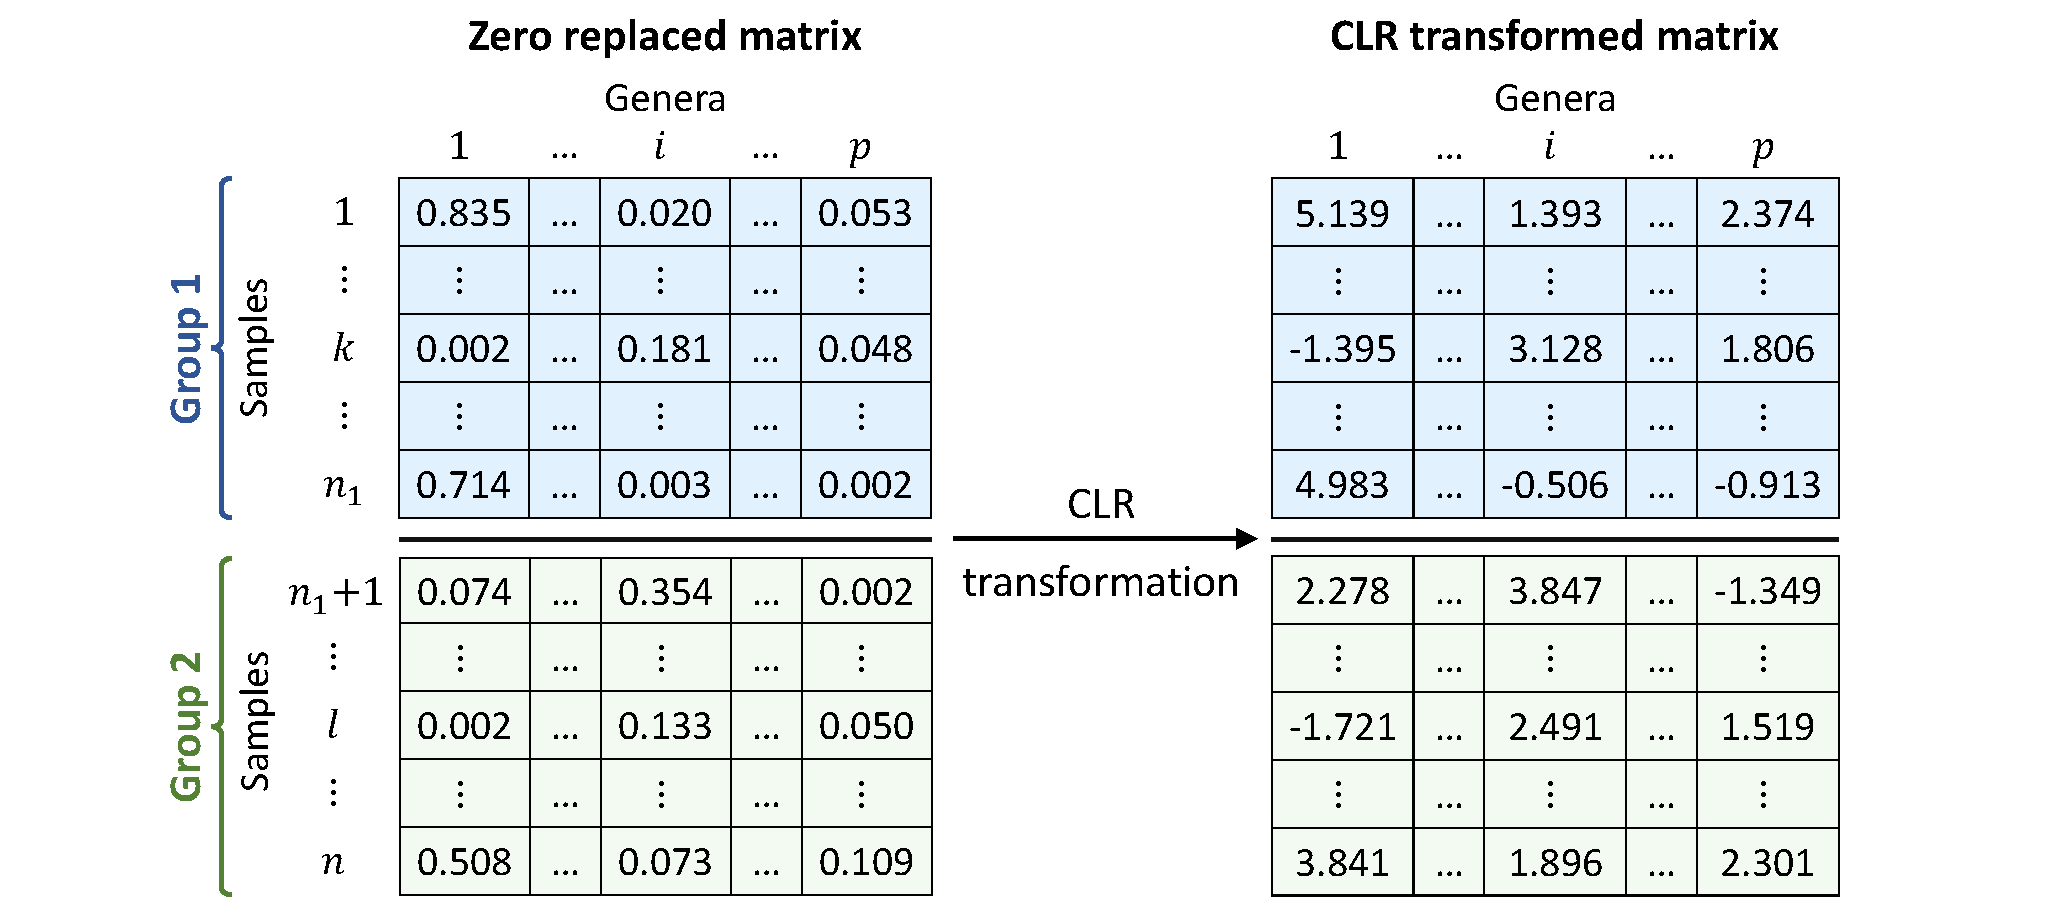
\includegraphics[width=\textwidth]{../ch02_microbiome_data/overview_figures/overview_transformation.pdf}
\caption{\textbf{Overview of transformation by the centered log-ratio (CLR).} The figure illustrates the transformation of a zero-replaced genus-level matrix to CLR coordinates. For each sample, the strictly positive entries are transformed by taking logarithms relative to the sample-wise geometric mean. The resulting CLR-transformed matrix contains real-valued log-ratio coordinates, which may be positive or negative and are no longer constrained to sum to one. Matrix entries are shown rounded to three decimal places. The two colored sample blocks represent two groups and are shown for consistency with later comparative analyses. The transformation itself is applied sample-wise and is not group-specific.}
\label{fig:2micro:overview_transformation}
\end{figure}

After filtering, library-size adjustment, and zero handling where needed, microbiome data may still require a representation that is better suited to the statistical analysis of interest. Transformations map the data into a new coordinate system or numerical scale. They may be used to stabilize the mean--variance relationship of count data, to reduce skewness, or to represent compositional observations in log-ratio coordinates. In contrast to normalization, transformations do not primarily aim to make library sizes comparable, but define the variables on which downstream models, distances, and test statistics are computed.

This distinction is important because the terms \emph{normalization} and \emph{transformation} are sometimes used interchangeably in the microbiome literature. As discussed in Section~\ref{sec:2micro:normalization}, normalization aims to reduce artifactual variation and to make measurements more comparable across samples \citep{weiss2017normalization}. Transformations, in contrast, map the data into a new space, often a Euclidean space, to facilitate statistical modeling but do not recover absolute abundance information from relative measurements \citep{quinn2019field}. As emphasized by \citet{quinn2019field}, transformations are not normalizations: transformed values must always be interpreted relative to the chosen reference or coordinate system.

In microbiome data analysis, two transformation goals are particularly relevant. First, transformations such as variance-stabilizing transformations aim to reduce the dependence between the mean and variance of count data, which can improve the behavior of methods that assume approximately homoscedastic observations. Second, log-ratio transformations address the compositional structure of sequencing data by representing samples through ratios between components rather than through raw counts or proportions. Figure~\ref{fig:2micro:overview_transformation} illustrates this second perspective for the centered log-ratio (CLR) transformation, which is the default transformation used in the CLR-based analyses of this thesis. These two perspectives are not mutually exclusive, but they target different statistical problems and lead to different interpretations of the transformed values.

%====================================
\subsection{Variance-stabilizing transformations}
\label{sec:2micro:norm:vst}
%====================================

Beyond library size adjustment, transformations have been proposed that aim to stabilize the variance of count data in the presence of overdispersion. 
Such methods primarily address goal (2), namely the dependence of the variance on the mean.

For sequencing counts, the variance typically increases with the expected value. 
Under a Poisson model, $\mathrm{Var}(X)=\mathbb{E}(X)$, while under negative binomial models commonly used for high-throughput sequencing data, the variance satisfies
\begin{equation}
\mathrm{Var}(X) = \mu + \alpha \mu^2,
\end{equation}
where $\mu$ denotes the mean and $\alpha>0$ is a dispersion parameter \citep{anders2010differential,robinson2010edger}. 
This mean–variance relationship induces heteroscedasticity that can distort distance-based analyses, clustering, and linear modeling.

Variance-stabilizing transformations seek a function $h(\cdot)$ such that
\begin{equation}
\mathrm{Var}\!\big(h(X)\big)
\approx \text{constant}.
\end{equation}

Within the \texttt{DESeq2} framework, a variance-stabilizing transformation is obtained by estimating the mean--dispersion relationship and applying a transformation of the general form \citep{love2014moderated}
\begin{equation}
\mathrm{VST}(x_{ki}) = \int^{x_{ki}} \frac{d\mu}{\sqrt{v(\mu)}},
\end{equation}
where $v(\mu)$ denotes the estimated mean–variance function. 
In practice, $v(\mu)$ is estimated from the data, and the transformation is applied to size-factor–normalized counts.

The VST transformation yields approximately homoscedastic values that can improve the behavior of clustering, ordination, and other exploratory analyses based on Euclidean geometry.
Unlike log-ratio transformations, however, VST does not explicitly account for the compositional constraint induced by closure.

In a systematic comparison of normalization and transformation methods for microbiome data, \citet{badri2020shrinkage} showed that correlation structures obtained after applying VST were similar to those obtained using the CLR transformation. 
In particular, \citet{badri2020shrinkage} found that Pearson correlation estimates obtained after VST were similar to those obtained after CLR transformation in the settings considered.
Thus, although VST is motivated by variance stabilization rather than compositional geometry, it may yield correlation patterns similar to CLR-based analyses in some settings.

%====================================
\subsection{Log-ratio transformations}
\label{sec:2micro:norm:log-ratios}
%====================================

A principled approach to the statistical analysis of compositional data was developed by \citet{aitchison1982statistical}, who argued that inference should be based on ratios between components rather than on the raw parts themselves. 
Because closure induces a constant-sum constraint, the components of a composition are inherently dependent (Section~\ref{sec:2micro:charact:compositionality}). 
Standard summaries such as means, variances, correlations, and regression coefficients computed directly on proportions are therefore generally subcompositionally incoherent \citep{aitchison1982statistical,aitchison1986statistical}. 

For each sample $k$, let
$\mathbf{x}_k = (x_{k1}, \dots, x_{kp})^\top$
denote its composition after closure to a constant sum. 
Forming ratios between two components removes the influence of the total sum. 
For taxa $i$ and $j$ in sample $k$, the ratio is given by
\begin{equation}
\frac{x_{ki}}{x_{kj}}.
\end{equation}
This ratio is invariant under multiplication of the entire composition by a positive constant and remains unchanged under closure. 
Ratios therefore isolate the relative information contained in the data and are invariant under scaling. Moreover, the ratio between two retained components is unchanged when additional components are removed from the composition  \citep{aitchison1982statistical,greenacre2021compositional}.

Ratios operate on a multiplicative scale. 
Taking logarithms converts multiplicative relationships into additive ones and yields Euclidean coordinate representations of the simplex in which conventional multivariate methods can be formulated \citep{aitchison1986statistical,greenacre2021compositional}. 

However, all log-ratio transformations require strictly positive components. Their application to sparse microbiome count data therefore requires either a prior zero-handling step or a transformation specifically designed for zero-containing data, as discussed in Section~\ref{sec:2micro:clr_with_zeros}.

Within Aitchison's framework and subsequent developments, several log-ratio transformations have been proposed. The most commonly used are the following.

%------------------------------------
\subsubsection*{Additive log-ratio transformation (ALR).}
%------------------------------------

The additive log-ratio (ALR) transformation expresses each component relative to a chosen reference taxon, say taxon $p$. 
For sample $k$, it is defined as
\begin{equation}
\label{eq:2micro:ALR}
\text{ALR}(\mathbf{x}_k)_i = \log \frac{x_{ki}}{x_{kp}},
\qquad i = 1,\dots,p-1.
\end{equation}

The ALR transformation yields a full-rank $(p-1)$-dimensional representation in $\mathbb{R}^{p-1}$ and is computationally straightforward. 
Because the transformed variables are unconstrained, standard regression and multivariate models can be formulated directly in ALR form \citep{aitchison1982statistical,aitchison1986statistical}. 

However, ALR depends on the choice of reference component and is therefore not permutation invariant. Moreover, Euclidean distances computed after ALR transformation do not generally coincide with Aitchison distances in the simplex \citep{aitchison1986statistical}. In microbiome applications, selecting such a reference can be difficult because a taxon should ideally be prevalent, stably measured, and scientifically interpretable across all samples.

%------------------------------------
\subsubsection*{Centered log-ratio transformation (CLR).}
%------------------------------------

To avoid the asymmetry induced by selecting a single reference, Aitchison proposed the centered log-ratio (CLR) transformation \citep{aitchison1986statistical}. 
For sample $k$, it is defined as
\begin{equation}
\label{eq:2micro:CLR}
\text{CLR}(\mathbf{x}_k)_i = \log \frac{x_{ki}}{g(\mathbf{x}_k)},
\qquad i = 1,\dots,p,
\end{equation}
where the geometric mean is
\begin{equation}
\label{eq:2micro:geometric_mean}
g(\mathbf{x}_k) = \left( \prod_{i=1}^{p} x_{ki} \right)^{1/p}.
\end{equation}

The geometric mean treats all taxa symmetrically, so that each CLR coordinate represents a component relative to the geometric mean of all components in the sample.
The CLR transformation satisfies
\begin{equation}
\sum_{i=1}^{p} \text{CLR}(\mathbf{x}_k)_i = 0,
\end{equation}
so that CLR-transformed data lie in a $(p-1)$-dimensional subspace of $\mathbb{R}^{p}$. 
Consequently, the CLR covariance matrix is singular. 
Nevertheless, the Aitchison distance between two compositions equals the Euclidean distance between their CLR-transformed representations \citep{aitchison1986statistical}. 

%------------------------------------
\subsubsection*{Isometric log-ratio transformation (ILR).}
%------------------------------------

The isometric log-ratio (ILR) transformation \citep{egozcue2003isometric} constructs $(p-1)$ orthonormal log-contrasts, typically defined through a sequential binary partition of the taxa. 
In general form, the $j$th ILR component for sample $k$ is
\begin{equation}
z_{kj} = \sqrt{\frac{r_j s_j}{r_j + s_j}}
\log\frac{\left( \prod_{i \in R_j} x_{ki} \right)^{1/r_j}}{
\left( \prod_{i \in S_j} x_{ki} \right)^{1/s_j}},
\qquad j = 1,\dots,p-1,
\end{equation}
where $R_j$ and $S_j$ partition the taxa into two non-overlapping groups of sizes $r_j$ and $s_j$ \citep{greenacre2021compositional}. 

The ILR transformation produces orthonormal log-contrasts with respect to the Aitchison geometry. 
In contrast to CLR, the resulting covariance matrix is nonsingular, and Euclidean distances in ILR space exactly equal Aitchison distances between compositions \citep{egozcue2003isometric,greenacre2021compositional}. 

%------------------------------------
\subsubsection*{Practical considerations.}
%------------------------------------

The choice between ALR, CLR (and its variants), and ILR depends on the inferential objective:
\begin{itemize}
    \item ALR may be appropriate when a scientifically meaningful and stable reference taxon exists,
    \item CLR provides a symmetric representation and is widely used in exploratory microbiome analyses and network inference,
    \item ILR provides an orthonormal and full-rank Euclidean representation of Aitchison geometry and is therefore useful when unconstrained covariance estimation or standard multivariate modeling is required. However, interpretation depends on the chosen orthonormal basis, which can complicate applied interpretation \citep{egozcue2003isometric,greenacre2021compositional}.
\end{itemize}

Importantly, none of these transformations recover absolute abundances. All inference remains relative: differences between samples or groups must be interpreted with respect to ratios between taxa, or to a taxon relative to the chosen log-ratio reference, rather than as changes in absolute abundance \citep{quinn2019field}.

%%%%%%%%%%%%%%%%%%%%%%%%%%%%%%%%%%%%%
s\section{CLR transformations in the presence of zeros}
\label{sec:2micro:clr_with_zeros}
%%%%%%%%%%%%%%%%%%%%%%%%%%%%%%%%%%%%%

The preceding sections considered zero handling and log-ratio transformations as separate preprocessing problems. In practice, however, these two issues are tightly coupled. The CLR transformation is attractive for microbiome data because it represents each component relative to the geometric mean of the full composition and maps compositional data to a Euclidean space. At the same time, it requires strictly positive values and is therefore not directly applicable to sparse microbiome count matrices. Consequently, any CLR-based analysis of sequencing data requires a decision about how zeros are handled before or during transformation.

This section focuses on CLR-based representations because they play a central role in the analyses performed later in this thesis. In the application chapter, the CLR transformation is used whenever an analysis method allows the transformation to be chosen freely. This does not imply that CLR is universally preferable or that zero handling has a unique optimal solution. Rather, the aim is to make the consequences of this choice explicit and to compare different ways of combining zero handling with CLR-type transformations.

The following subsections therefore investigate several approaches, including global offset addition, multiplicative replacement before CLR transformation, and modified CLR variants that avoid replacing zeros directly. For each approach, we discuss the underlying idea, its advantages, and its limitations. This comparison provides the basis for the preprocessing choices used in the later chapters and clarifies which statistical interpretation is attached to the transformed microbiome data.

%====================================
\subsection{CLR after multiplicative replacement} 
\label{sec:2micro:clr_with_zeros:multRepl}
%====================================

A common way to make the CLR transformation applicable to sparse microbiome data is to first replace zeros by small positive values and subsequently apply the standard CLR transformation to the resulting strictly positive composition. Among the replacement strategies introduced in Section~\ref{sec:2micro:zeros:replacement}, multiplicative replacement is particularly compatible with the log-ratio interpretation of the CLR transformation, because it preserves ratios among originally non-zero components.

Let $\mathbf{x}_k^\ast$ denote the multiplicatively replaced version of sample $\mathbf{x}_k$. The CLR transformation is then given by
\begin{equation}
\operatorname{CLR}(\mathbf{x}_k^\ast)_i=\log\left(\frac{x_{ki}^\ast}{g(\mathbf{x}_k^\ast)}\right),
\label{eq:2micro:clr_after_mult_replacement}
\end{equation}
where $g(\mathbf{x}_k^\ast)$ denotes the geometric mean of the components of $\mathbf{x}_k^\ast$.

The relevance of multiplicative replacement becomes clear from the relationship between CLR coordinate differences and pairwise log-ratios. If $x_{ki}>0$ and $x_{kj}>0$, multiplicative replacement changes both components by the same sample-specific factor, so that
\begin{equation}
\frac{x_{ki}^\ast}{x_{kj}^\ast}=\frac{x_{ki}}{x_{kj}}.
\label{eq:2micro:mult_replacement_ratio_preservation}
\end{equation}
Since differences between CLR coordinates are pairwise log-ratios,
\begin{equation}
\operatorname{CLR}(\mathbf{x}_k^\ast)_i-\operatorname{CLR}(\mathbf{x}_k^\ast)_j
=
\log\left(\frac{x_{ki}^\ast}{x_{kj}^\ast}\right),
\label{eq:2micro:clr_difference_logratio}
\end{equation}
the observed log-ratios between non-zero components are retained after transformation. This property is important for analyses whose interpretation depends directly on log-ratio geometry, including Aitchison distances, proportionality, and CLR-based association measures.

At the same time, multiplicative replacement is still a replacement procedure and therefore introduces assumptions about the unobserved zero components. The magnitude of the replacement value influences the transformed values assigned to zeros and can affect distances or associations involving sparse taxa. Thus, multiplicative replacement followed by CLR should not be interpreted as recovering the unobserved true composition. Rather, it provides a zero-aware approximation to the standard CLR representation that preserves ratios among components that were actually observed.

%====================================
\subsection{Modified CLR (mCLR)} 
\label{sec:2micro:clr_with_zeros:mCLR}
%====================================

The modified centered log-ratio transformation (mCLR) was proposed in the context of sparse microbial graphical modeling, in particular for the SPRING framework of \citet{yoon2019microbial}. In contrast to replacement-based approaches, mCLR does not replace zero counts by positive values before transformation. Instead, it computes the geometric mean only over the positive components of each sample and leaves zero components unchanged.

For a sample $\mathbf{x}_k=(x_{k1},\ldots,x_{kp})^\top$, let $P_k=\{i:x_{ki}>0\}$ denote the index set of positive components, and let $\mathbf{x}_k^+=(x_{ki}:i\in P_k)^\top$ denote the corresponding positive subvector. The ordinary geometric mean of the positive components is
\begin{equation}
g(\mathbf{x}_k^+)=\left(\prod_{i\in P_k}x_{ki}\right)^{1/|P_k|}.
\label{eq:2micro:positive_geometric_mean}
\end{equation}
The mCLR transformation is defined as
\begin{equation}
\operatorname{mCLR}(\mathbf{x}_k)_i=
\begin{cases}
0, & x_{ki}=0,\\
\log\left(\frac{x_{ki}}{g(\mathbf{x}_k^+)}\right)+\varepsilon_k, & x_{ki}>0,
\end{cases}
\label{eq:2micro:mclr}
\end{equation}
where $\varepsilon_k>0$ is a sample-specific shift constant chosen such that all transformed non-zero values are positive.

The main advantage of mCLR is that it avoids explicit zero replacement and preserves the distinction between zero and non-zero components. Moreover, for two positive components $x_{ki}>0$ and $x_{kj}>0$, both the positive-part geometric mean and the common sample-specific shift cancel when coordinate differences are formed:
\begin{equation}
\log\left(\frac{x_{ki}}{g(\mathbf{x}_k^+)}\right)
-
\log\left(\frac{x_{kj}}{g(\mathbf{x}_k^+)}\right)
=
\log\left(\frac{x_{ki}}{x_{kj}}\right).
\label{eq:2micro:mclr_positive_logratio}
\end{equation}
Thus, mCLR preserves log-ratios between components that are both positive within the same sample.

However, this within-sample property does not imply that mCLR is generally interchangeable with the standard CLR transformation. The reference $g(\mathbf{x}_k^+)$ depends on the sample-specific zero pattern, zeros remain fixed at zero, and the shift $\varepsilon_k$ is also sample-specific. Consequently, the transformed value of a taxon depends not only on its own count, but also on the sample-specific set of positive components and on the corresponding shift. This can affect distances between samples, marginal distributions of transformed taxa, and regression-type or group-comparison analyses.

For this reason, mCLR is best understood as a method-specific transformation rather than as a general zero-handling strategy for CLR-based analyses. It is appropriate when the downstream method explicitly defines or assumes this representation, as in SPRING, where mCLR is combined with a semi-parametric rank-based graphical modeling approach that can handle a large amount of zeros in the data. In this thesis, mCLR is therefore discussed as a method-specific alternative to replacement-based CLR, but it is not used when a standard CLR or Aitchison interpretation is required.

%====================================
\subsection{Geometric mean extension and offset-based CLR}
\label{sec:2micro:clr_with_zeros:gmeCLR}
%====================================

The geometric mean is the central reference quantity in the CLR transformation. This makes extensions of the geometric mean to data containing zeros an intuitively appealing starting point for adapting CLR-based transformations to sparse data. A formal extension of the geometric mean was proposed by \citet{delacruz2019geometric}. This extension was not originally introduced as a CLR transformation, but as a modification of the geometric mean that remains well-defined when some components are zero. Since the standard CLR transformation is undefined in the presence of zeros because both the geometric mean and the component-wise logarithms cannot be evaluated in the usual way, it is natural to ask whether such an extended geometric mean can contribute to handling zeros in CLR-based analyses.

Using the notation from Equation~\eqref{eq:2micro:positive_geometric_mean}, let $\mathbf{x}_k^+$ denote the positive subvector of sample $k$, and let $g(\mathbf{x}_k^+)$ be the ordinary geometric mean of its positive components. For a candidate offset $\delta>0$, the extended geometric mean of the full sample is defined as
\begin{equation}
\tilde{g}_{\delta}(\mathbf{x}_k)=\exp\left(\frac{1}{p}\sum_{i=1}^p\log(x_{ki}+\delta)\right)-\delta.
\label{eq:2micro:extended_geometric_mean}
\end{equation}
The subtraction of $\delta$ maps the shifted geometric mean back to the original scale and is the defining feature of the extended geometric mean. Analogously, the extended geometric mean of the positive part is denoted by $\tilde{g}_{\delta}(\mathbf{x}_k^+)$.

Following \citet{delacruz2019geometric}, the offset is chosen such that the extended geometric mean remains close to the ordinary geometric mean when evaluated on the positive components only. For a tolerance parameter $\epsilon>0$, the sample-specific offset is defined as
\begin{equation}
\delta_k=\sup\left\{\delta>0:\left|\tilde{g}_{\delta}(\mathbf{x}_k^+)-g(\mathbf{x}_k^+)\right|\leq \epsilon\, g(\mathbf{x}_k^+)\right\}.
\label{eq:2micro:extended_geometric_mean_delta}
\end{equation}
Thus, $\delta_k$ is the supremum of offsets for which the extended geometric mean of the positive components deviates from $g(\mathbf{x}_k^+)$ by at most the relative tolerance $\epsilon$. Smaller values of $\epsilon$ enforce closer agreement with the ordinary geometric mean and lead to smaller offsets, whereas larger values allow stronger regularization. The construction therefore provides a principled way to choose an offset whose effect on the geometric mean of the observed positive components is controlled.

However, solving the geometric-mean problem does not by itself solve the zero problem of the CLR transformation. Even if $\tilde{g}_{\delta}(\mathbf{x}_k)$ is well-defined, the expression $\log(x_{ki}/\tilde{g}_{\delta}(\mathbf{x}_k))$ remains undefined for components with $x_{ki}=0$. A zero-aware CLR-type transformation therefore still requires a modification of the components entering the logarithm. In the microbiome context, \citet{mishra2025variational} used the offset obtained from the geometric mean extension as an additive replacement before applying a CLR-type transformation. In the notation used here, this can be written as
\begin{equation}
\operatorname{clr}_{\delta_k}^{(+)}(\mathbf{x}_k)_i=
\log\left(\frac{x_{ki}+\delta_k}{\tilde{g}_{\delta_k}(\mathbf{x}_k)+\delta_k}\right),
\qquad i=1,\ldots,p.
\label{eq:2micro:offset_based_clr}
\end{equation}
Since $\tilde{g}_{\delta_k}(\mathbf{x}_k)+\delta_k$ is the ordinary geometric mean of the shifted vector $\mathbf{x}_k+\delta_k$, Equation~\eqref{eq:2micro:offset_based_clr} is equivalent to applying the standard CLR transformation after adding $\delta_k$ to all components. This yields a finite CLR vector in the zero-sum subspace of $\mathbb{R}^p$ and avoids undefined logarithms.

The drawback of this construction is that the offset is added not only to zero components, but also to components that were already observed. Consequently, ratios among originally non-zero components are changed. For two positive components $x_{ki}>0$ and $x_{kj}>0$, the original log-ratio is
\begin{equation}
\log\left(\frac{x_{ki}}{x_{kj}}\right),
\label{eq:2micro:original_positive_logratio}
\end{equation}
whereas the corresponding log-ratio after additive offset replacement is
\begin{equation}
\log\left(\frac{x_{ki}+\delta_k}{x_{kj}+\delta_k}\right).
\label{eq:2micro:offset_positive_logratio}
\end{equation}
The two quantities are generally not equal. Thus, the offset-based transformation does not only regularize zeros, but also perturbs relative information among taxa that were already observed. This is particularly relevant for analyses whose interpretation depends on log-ratio geometry, such as Aitchison distances, CLR-based association measures, proportionality analysis, or group comparisons on a log-ratio scale.

One might consider using the offset $\delta_k$ from Equation~\eqref{eq:2micro:extended_geometric_mean_delta} only to replace zero components, while leaving positive components unchanged. Such a strategy would preserve ratios among originally non-zero taxa. However, this would no longer correspond to the original geometric mean extension. The offset $\delta_k$ is calibrated by studying how adding $\delta$ to the positive components changes their geometric mean. If the offset is subsequently applied only to zeros, the criterion in Equation~\eqref{eq:2micro:extended_geometric_mean_delta} no longer describes the distortion induced by the actual replacement rule. In that case, $\delta_k$ would merely be used as a data-adaptive zero-replacement value, and the link to the extended geometric mean construction would be largely lost. Developing and evaluating such a modified replacement strategy would constitute a separate methodological problem and is outside the scope of this thesis.

The geometric mean extension therefore highlights an important trade-off. Adding an offset to all components stabilizes the logarithm and yields a complete CLR-type representation, but it changes ratios among originally non-zero taxa. Replacing only zeros preserves these ratios, but then the offset can no longer be justified directly by the extended geometric mean criterion. For this reason, the geometric mean extension is best viewed as a useful attempt to address one part of the zero problem in CLR-based transformations, but not as a general solution to zero handling in CLR-based microbiome analysis. In this thesis, offset-based CLR transformations motivated by the geometric mean extension are therefore not used as the primary representation for inferential analyses. Instead, multiplicative replacement followed by CLR is used when a standard log-ratio or Aitchison interpretation is required, while offset-based transformations may be considered as smoothed sensitivity representations in settings where extreme zero-induced values are of particular concern.

%====================================
\subsection{Comparative example}
\label{sec:2micro:clr_with_zeros:example}
%====================================

The preceding subsections introduced different ways of making CLR-based transformations applicable to data containing zeros: applying CLR after multiplicative replacement, modifying the CLR transformation through mCLR, and using an additive offset motivated by the extended geometric mean. These approaches solve the computational problem of undefined logarithms in different ways, but they do not preserve the same relative information. The zero-replacement strategies discussed in Section~\ref{sec:2micro:zeros:replacement} already showed that multiplicative replacement preserves ratios among originally non-zero components, whereas adding a pseudo-count to all components changes these ratios. Since the CLR transformation is defined through division by the geometric mean rather than by direct pairwise division of taxa, it may not be immediately obvious how this difference propagates to CLR-transformed data. However, differences between CLR coordinates are pairwise log-ratios, and downstream analyses based on CLR-transformed data therefore remain sensitive to changes in the underlying ratios.

The following toy example illustrates how multiplicative replacement and additive offset replacement can lead to different results in common downstream analyses, including distance-based analysis, differential distribution analysis, feature-level group contrasts, and association or proportionality analysis. The example is deliberately small and is intended as a diagnostic illustration rather than as a performance comparison. To focus on the effect of zero handling, all samples in the toy data have the same total count. In real microbiome analyses, where sequencing depths usually differ between samples, counts should first be brought to a common compositional scale before zero replacement so that the replacement value has the same relative influence in each sample.

Consider the small count data set in Table~\ref{tab:toy_zero_example_original}. The first two samples belong to group $A$, the last two samples belong to group $B$. Taxon 2 is doubled in group $B$ compared with group $A$, taxon 3 is decreased accordingly because all samples have the same total count, and taxon 1 contains zeros. In the following, let $\mathbf{X}=(x_{ki})$ denote the count table in Table~\ref{tab:toy_zero_example_original}, where $\mathbf{x}_k=(x_{k1},x_{k2},x_{k3})^\top$ is the count vector of sample $k$. The corresponding group labels are denoted by $\mathbf{g}=(g_1,\ldots,g_4)^\top$, with $g_k\in\{A,B\}$. For simplicity, let $\delta=1$, where $\delta$ denotes the small positive replacement or offset value used in the two transformations. Superscript $(M)$ denotes values after multiplicative replacement, whereas superscript $(+)$ denotes values after additive offset replacement.

\begin{table}[ht]
\centering
\caption{Toy example used to compare multiplicative replacement and additive offset replacement before CLR transformation. All samples have the same total count.}
\label{tab:toy_zero_example_original}
\begin{tabular}{llrrrr}
\toprule
Sample & Group & Taxon 1 & Taxon 2 & Taxon 3 & $\Sigma$ \\
\midrule
S1 & A & 0 & 4 & 96 & 100 \\
S2 & A & 1 & 4 & 95 & 100 \\
S3 & B & 0 & 8 & 92 & 100 \\
S4 & B & 1 & 8 & 91 & 100 \\
\bottomrule
\end{tabular}
\end{table}

Using the replacement strategies introduced in Section~\ref{sec:2micro:zeros:replacement}, the data after multiplicative replacement and additive offset replacement are shown in Tables~\ref{tab:toy_zero_example_mult_replacement} and~\ref{tab:toy_zero_example_additive_offset}, respectively. Multiplicative replacement preserves the original sample totals by proportionally rescaling the positive components, whereas additive offset replacement adds $\delta$ to all three taxa and therefore increases each sample total by $3$.

\begin{table}[ht]
\centering
\caption{Toy data after multiplicative replacement with $\delta=1$. Zeros are replaced by $\delta$, and positive components are rescaled so that the sample sum is preserved.}
\label{tab:toy_zero_example_mult_replacement}
\begin{tabular}{llrrrr}
\toprule
Sample & Group & Taxon 1 & Taxon 2 & Taxon 3 & $\Sigma$ \\
\midrule
S1 & A & 1.00 & 3.96 & 95.04 & 100 \\
S2 & A & 1.00 & 4.00 & 95.00 & 100 \\
S3 & B & 1.00 & 7.92 & 91.08 & 100 \\
S4 & B & 1.00 & 8.00 & 91.00 & 100 \\
\bottomrule
\end{tabular}
\end{table}

\begin{table}[ht]
\centering
\caption{Toy data after additive offset replacement with $\delta=1$. The offset is added to all components, so the sample sum increases by $3$.}
\label{tab:toy_zero_example_additive_offset}
\begin{tabular}{llrrrr}
\toprule
Sample & Group & Taxon 1 & Taxon 2 & Taxon 3 & $\Sigma$ \\
\midrule
S1 & A & 1 & 5 & 97 & 103 \\
S2 & A & 2 & 5 & 96 & 103 \\
S3 & B & 1 & 9 & 93 & 103 \\
S4 & B & 2 & 9 & 92 & 103 \\
\bottomrule
\end{tabular}
\end{table}

Figure~\ref{fig:2micro:clr_toy_example} visualizes the original counts and the CLR-transformed values after the two replacement strategies. The most important observation is that near-equality in the original counts is largely preserved after multiplicative replacement followed by CLR, but not after additive offset replacement followed by CLR. In the original data, the two samples within each group have identical counts for taxon 2 and only small differences for taxon 3. After multiplicative replacement, the corresponding CLR values remain very close. After additive offset replacement, however, the CLR values separate more strongly, even for taxa that contain no zeros. This reflects the fact that adding an offset to all components changes ratios among originally non-zero taxa and can therefore introduce additional variation into the transformed representation.

\begin{figure}[!htb]
\centering
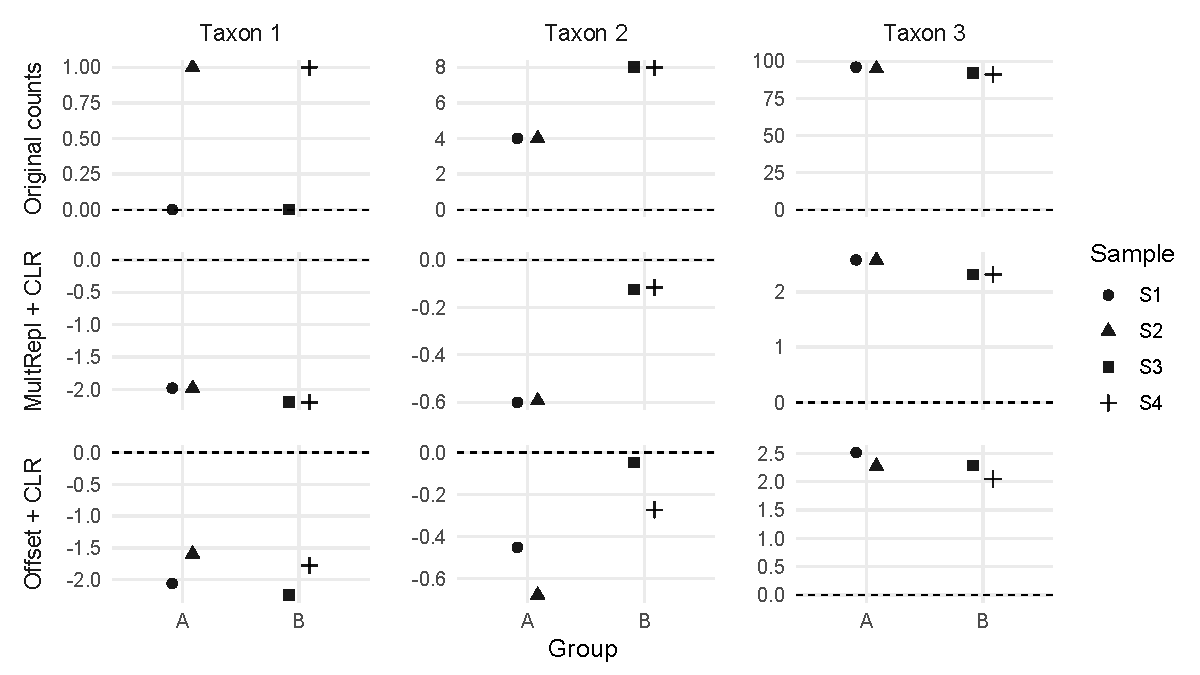
\includegraphics[width=\textwidth]{../ch02_microbiome_data/figures/clr_mini_example/thesis_original_transformed_values-1.pdf}
\caption{\textbf{Visualization of the toy data before and after CLR transformation.} The first row shows the original counts. The second and third rows show CLR-transformed values after multiplicative replacement (``multRepl + CLR'') and additive offset replacement (``Offset + CLR''), respectively. Multiplicative replacement changes positive components only through a proportional rescaling within samples, whereas additive offset replacement adds the same value to all components. Consequently, the transformed values differ not only for the taxon containing zeros, but also for taxa that were positive in all samples.}
\label{fig:2micro:clr_toy_example}
\end{figure}

For \textbf{distance-based analyses}, the relevant object is the geometry between samples in CLR space. Consider the first two samples, which differ by a maximum of one in their original counts. Their CLR distance after multiplicative replacement is
\begin{equation}
\left\|\operatorname{CLR}(x_1^{(M)})-\operatorname{CLR}(x_2^{(M)})\right\|_2 \approx 0.008.
\label{eq:2micro::mult_replacement_distance_example}
\end{equation}
After additive offset replacement, the corresponding distance is
\begin{equation}
\left\|\operatorname{CLR}(x_1^{(+)})-\operatorname{CLR}(x_2^{(+)})\right\|_2 \approx 0.570.
\label{eq:2micro:additive_offset_distance_example}
\end{equation}
Thus, the offset strategy leads to a substantially larger distance between the same two samples. The reason is that additive offset replacement changes ratios among observed components, whereas multiplicative replacement changes positive components only through a proportional rescaling. This example does not imply that multiplicative replacement eliminates the influence of zeros on distances. The replacement value and the sample-specific zero pattern can still affect CLR coordinates. Its advantage is more specific: it preserves ratios among components that were originally observed within a sample. In the toy example, the comparison between S1 and S2 is especially close after multiplicative replacement because both samples have the same total count and the replacement results in almost identical compositions. In real data, samples usually differ in sequencing depth and zero pattern. Therefore, normalization to a common compositional scale and suitable filtering remain important before applying CLR-based distance analyses.

For \textbf{differential distribution analyses}, the transformed values themselves are the objects being compared. Consider taxon 2. After multiplicative replacement followed by CLR, the transformed values are
\begin{equation}
\operatorname{CLR}(x^{(M)})_{\cdot 2}
\approx
(-0.601,\,-0.594,\,-0.124,\,-0.117),
\label{eq:2micro:mult_replacement_taxon2_clr_values}
\end{equation}
whereas after additive offset replacement followed by CLR they are
\begin{equation}
\operatorname{CLR}(x^{(+)})_{\cdot 2}
\approx
(-0.452,\,-0.680,\,-0.046,\,-0.273).
\label{eq:2micro:additive_offset_taxon2_clr_values}
\end{equation}
Thus, the marginal distribution of the CLR-transformed values of taxon 2 differs between the two replacement strategies, even though the same original count table is used. This is relevant for analyses that compare transformed taxon-level distributions across samples or groups.

The same transformed values would also enter a simple feature-level \textbf{differential abundance-style comparison} on the CLR scale. For taxon 2, the difference between the mean transformed value in group $B$ and the mean transformed value in group $A$ is
\begin{equation}
\Delta_2^{(M)}
=
\frac{1}{2}\sum_{k:g_k=B}\operatorname{CLR}(\mathbf{x}_k^{(M)})_2
-
\frac{1}{2}\sum_{k:g_k=A}\operatorname{CLR}(\mathbf{x}_k^{(M)})_2
\approx 0.476
\label{eq:2micro:mult_replacement_da_contrast_example}
\end{equation}
after multiplicative replacement, whereas after additive offset replacement it is
\begin{equation}
\Delta_2^{(+)}
=
\frac{1}{2}\sum_{k:g_k=B}\operatorname{CLR}(\mathbf{x}_k^{(+)})_2
-
\frac{1}{2}\sum_{k:g_k=A}\operatorname{CLR}(\mathbf{x}_k^{(+)})_2
\approx 0.406.
\label{eq:2micro:additive_offset_da_contrast_example}
\end{equation}
This calculation is not intended as a realistic differential abundance test, because the toy data contain only two samples per group. It nevertheless illustrates that the transformed group difference entering such an analysis can depend on the zero-handling strategy before any statistical test is performed. The toy example is balanced in the sense that both groups contain one sample with a zero in taxon 1 and one sample without such a zero. In real data, zero patterns are usually not balanced across samples or groups, so the influence of replacement on group comparisons may be stronger and less transparent.

For \textbf{association and proportionality analyses}, pairwise log-ratios and their variation across samples are central. Consider taxa 2 and 3, which are positive in all four samples. In the original data, the corresponding sample-wise log-ratios are
\begin{equation}
\log\left(\frac{x_2}{x_3}\right)
\approx
(-3.178,\,-3.168,\,-2.442,\,-2.431).
\label{eq:2micro:original_logratio_taxa23_example}
\end{equation}
After multiplicative replacement, the CLR-transformed values of taxa 2 and 3 change because the geometric mean is affected by the zero replacement. However, their coordinate differences remain identical to the original log-ratios:
\begin{equation}
\operatorname{CLR}(x^{(M)})_{\cdot 2}
-
\operatorname{CLR}(x^{(M)})_{\cdot 3}
=
\log\left(\frac{x_2^{(M)}}{x_3^{(M)}}\right)
\approx
(-3.178,\,-3.168,\,-2.442,\,-2.431).
\label{eq:2micro:mult_replacement_logratio_taxa23_example}
\end{equation}
This equality holds because multiplicative replacement rescales originally non-zero components within a sample by the same factor and therefore preserves their ratios. In contrast, after additive offset replacement the corresponding coordinate differences become
\begin{equation}
\operatorname{CLR}(x^{(+)})_{\cdot 2}
-
\operatorname{CLR}(x^{(+)})_{\cdot 3}
=
\log\left(\frac{x_2^{(+)}}{x_3^{(+)}}\right)
\approx
(-2.965,\,-2.955,\,-2.335,\,-2.325).
\label{eq:2micro:additive_offset_logratio_taxa23_example}
\end{equation}
Thus, additive offset replacement changes the log-ratio pattern even for a pair of taxa that contains no zeros. For example, the variance of this log-ratio is approximately $0.181$ in the original data and remains $0.181$ after multiplicative replacement, whereas it decreases to approximately $0.132$ after additive offset replacement. Since association measures, proportionality measures, and network edges can depend on the variation of such log-ratios or transformed taxon profiles across samples, this modification can affect downstream inference.


This example illustrates why multiplicative replacement and additive offset replacement should not be treated as equivalent preprocessing choices. Multiplicative replacement preserves ratios among originally observed components and therefore remains closest to the standard CLR and Aitchison interpretation after zero replacement. Additive offset replacement yields a smoothed complete representation, but it changes ratios among non-zero components and can therefore affect distances, feature-level contrasts, marginal transformed distributions, and association patterns. This does not mean that multiplicative replacement is universally optimal. In particular, between-sample comparisons can still be affected by the replacement value and by sample-specific zero patterns. However, multiplicative replacement avoids additionally perturbing ratios among observed components, whereas additive offset replacement changes such ratios by construction.

The mCLR transformation is not included in this numerical comparison because it is not a replacement strategy in the same sense. It leaves zeros unchanged, centers only the positive components, and applies a sample-specific positive shift to non-zero transformed values. As discussed above, this representation can be appropriate when explicitly required by a method, but it should not be interpreted as an interchangeable substitute for standard CLR in comparative analyses.

The R code generating the tables, numerical values, and Figure~\ref{fig:2micro:clr_toy_example} is included in the thesis repository archived on Zenodo \citep{Peschel2026thesisRepo}. Within this repository, the material for the present section is provided in the folder \href{https://github.com/stefpeschel/phd_thesis/tree/main/ch02_microbiome_data}{\texttt{ch02\_microbiome\_data}}.

%====================================
\section{Statistical consequences of preprocessing}
\label{sec:2micro:preprocessing_consequences}
%====================================

From a statistical perspective, the preprocessing steps discussed in this chapter should not be viewed merely as technical data-cleaning procedures, but as integral components of the analysis strategy. Filtering, zero handling, normalization, and transformation determine the effective data representation on which downstream summaries, models, and hypothesis tests are based. They therefore influence not only numerical stability, but also the inferential target and the interpretation of the results.

Filtering changes both the number of samples and the number of features entering the analysis. Removing low-depth samples can reduce the influence of sampling zeros and stabilize distance-based analyses \citep{weiss2017normalization}, while filtering rare taxa can reduce the influence of features that contribute little information but many sampling zeros. At the same time, taxa filtering changes the subcomposition under study and therefore modifies the feature set and relative reference system on which compositional inference is based \citep{aitchison1986statistical}. This is particularly relevant when conclusions are interpreted as statements about the microbial community as a whole, although the analysis was performed only on a filtered subset of features.

Zero handling introduces additional assumptions because the biological or technical origin of an observed zero is generally not identifiable from the count table alone \citep{martin2011dealing,quinn2019field}. Replacement and imputation strategies determine how unobserved or undetected taxa enter log-ratio coordinates and can therefore affect variances, associations, distances, and network structures. Classical compositional data analysis distinguishes between replacement strategies that preserve the relative structure among observed components and approaches that perturb non-zero components \citep{martin-fernandez2003dealing}. More recently, \citet{tang2026critical} provided a comparison of zero-handling strategies for high-dimensional compositional count data and emphasized that simple replacement rules become less reliable when the proportion of zeros is high. In the settings considered, multiplicative replacement performed well when the zero proportion was moderate, whereas low-rank log-ratio imputation by lrSVD performed more favorably in highly sparse settings. This illustrates that zero handling is not simply a numerical workaround for logarithms, but a modeling decision about how sparse observations are represented statistically.

Normalization and transformation define the scale or coordinate system of the analysis. Scaling-based methods such as total sum scaling address heterogeneous library sizes but make the compositional constraint induced by closure explicit rather than resolving it \citep{weiss2017normalization,aitchison1986statistical}. This is also relevant before zero replacement: although the CLR transformation is scale-invariant for strictly positive data, the replacement value itself is not automatically comparable across samples with different library sizes. Therefore, when a zero-replacement method uses fixed replacement values, the data should first be brought to a common compositional scale, for example by total count normalization or conversion to relative abundances. Alternatively, the replacement procedure must account explicitly for sample-specific totals. Variance-stabilizing transformations primarily target the mean-variance relationship of count data, whereas log-ratio transformations embed compositional observations into Euclidean space and make inference interpretable in terms of ratios \citep{aitchison1986statistical,greenacre2021compositional}. Consequently, the same biological data may lead to different statistical objects depending on the chosen representation: scaled counts, variance-stabilized values, imputed compositions, or log-ratio coordinates.

These choices also affect hypothesis testing and network analysis. Permutation tests require exchangeability under the null hypothesis \citep{good2005permutation,phipson2010permutation}, and preprocessing can change the finite-sample behavior of the test statistic by altering sparsity, variance heterogeneity, or the effective feature space. This is particularly important when preprocessing contains a non-trivial imputation step. If an imputation method is considered part of the statistic, or if it is fitted separately within permuted groups, it should in principle be repeated under each permutation. For computationally intensive methods such as lrSVD, this can make permutation-based workflows substantially more complex. Association network analysis is especially sensitive to these decisions, because edge estimation depends on the conditioning, sparsity, and geometry of the transformed data \citep{kurtz2015sparse}. This motivates workflows that make preprocessing choices explicit and reproducible rather than treating them as hidden defaults.

Taken together, preprocessing defines the retained sample set, the feature space, and the coordinate representation in which community-level summaries, feature-level measures, and association networks are analyzed. It should therefore be understood as part of statistical inference for microbiome data rather than as a separate technical step preceding the actual analysis.

%====================================
\section{Preprocessing choices in this thesis}
\label{sec:2micro:preprocessing_choices_thesis}
%====================================

The preprocessing strategy used in this thesis follows from the statistical perspective outlined above. Preprocessing choices are not treated as neutral technical defaults, but as part of the definition of the data representation used for inference. At the same time, using consistent baseline choices whenever possible improves interpretability across analysis sections. Therefore, this thesis defines a general preprocessing framework that is adapted when required by the downstream analysis. Table~\ref{tab:2micro:preprocessing_choices} gives a compact overview of the default choices used throughout the thesis.

\begin{table}[!ht]
\centering
\caption{\textbf{Preprocessing choices in this thesis.} Summary of the default preprocessing choices used throughout the thesis. The step numbers indicate the default preprocessing order. Deviations from these choices or from this order are stated and justified in the corresponding analysis sections.}
\label{tab:2micro:preprocessing_choices}
\vspace{0.5em}
\renewcommand{\arraystretch}{1.3}
\begin{tabular}{p{4cm}p{10.6cm}}
\toprule
\textbf{Step} & \textbf{Choice in this thesis} \\
\midrule
\textbf{1. Sample filtering} & Remove samples with \textbf{zero total counts}. Apply additional sample filtering if required by the analysis. \\
\textbf{2. Taxa filtering} & Remove taxa with \textbf{zero total counts after sample filtering}. Apply additional prevalence or abundance filtering if required for stable estimation or interpretation. \\
\textbf{3. Aggregation} & Use \textbf{genus-level} aggregation unless stated otherwise. The choice of genus level is motivated in the application chapter after exploratory inspection of the ASV-level data. \\
\textbf{4. Normalization} & Use \textbf{total sum scaling}, i.e. conversion to relative abundances, when a common compositional scale is required. \\
\textbf{5. Zero handling} & Use \textbf{multiplicative replacement} as the default zero-handling strategy before CLR transformation. \\
\textbf{6. Transformation} & Use the \textbf{CLR transformation} for analyses requiring log-ratio coordinates or Aitchison geometry. \\
\bottomrule
\end{tabular}
\end{table}

As a minimal filtering step, samples and taxa with an overall count of zero are removed before analysis. Such samples or taxa do not contribute quantitative information and can lead to undefined quantities in relative abundance, log-ratio, or distance-based analyses. Further filtering is performed in an analysis-specific manner when needed. This is particularly important for highly sparse microbiome data, where zero handling can otherwise dominate the transformed representation. For example, network-based analyses often require more restrictive taxon filtering to obtain smaller and more interpretable networks and to reduce instability caused by extremely sparse taxa,whereas community-level analyses may retain a larger feature set when rare taxa are considered relevant to the chosen community summary. Thus, filtering is not fixed globally beyond the removal of empty samples and taxa, but is chosen according to the statistical and interpretational requirements of the analysis.

Taxonomic aggregation is also treated as an analysis decision rather than as a purely technical simplification. In this thesis, genus-level aggregation is used as the default representation unless stated otherwise. This choice provides a compromise between biological resolution and statistical stability. In the PASTURE application, the decision to work at genus level is made after an exploratory description of the ASV-level data and the sparsity structure across taxonomic levels.

For the CLR-based workflow used in this thesis, the data are first brought to a common compositional scale by total sum scaling, or equivalently by conversion to relative abundances, before multiplicative replacement is applied. This step ensures that the replacement value has a comparable compositional meaning across samples with different sequencing depths. After this normalization step, multiplicative replacement followed by CLR transformation is used as the default representation, unless a different zero-handling strategy is explicitly motivated by the downstream method or analysis target. This choice is motivated by Sections~\ref{sec:2micro:zeros:replacement} and~\ref{sec:2micro:clr_with_zeros}. Multiplicative replacement makes the CLR transformation applicable to sparse data while preserving ratios among originally non-zero components. This property is important because differences between CLR coordinates are pairwise log-ratios, and many analyses considered in this thesis depend directly or indirectly on such log-ratio relationships. For Aitchison-distance-based analyses, the transformed values define the geometry between samples. For exploratory feature-level analyses conducted on the CLR scale, the transformed values define taxon-specific marginal distributions or group contrasts. For proportionality analyses and several compositional association approaches, log-ratio relationships and their variation across samples are central.

This default should not be interpreted as a claim that multiplicative replacement is universally optimal. In very sparse data sets, more elaborate imputation approaches such as lrSVD may exploit low-rank structure across samples and taxa and may perform better than simple replacement rules \citep{tang2026critical}. However, lrSVD introduces additional modeling assumptions and tuning choices, including the choice of rank and the treatment of bounds for censored or missing values. It also complicates permutation-based analyses, which are a central methodological theme of this thesis. When lrSVD is estimated from the analyzed data, it should generally be repeated within each permutation so that the permutation procedure reflects the complete analysis pipeline. In the permutation-intensive analyses considered in this thesis, this would substantially increase computational cost and add an additional methodological layer outside the present scope. For this reason, lrSVD is discussed as an important alternative for highly sparse compositional count data, but it is not used as the primary zero-handling strategy here.

Other alternatives are also interpreted more narrowly. Offset-based CLR transformations motivated by the extended geometric mean provide a smoothed complete representation and may reduce extreme zero-induced transformed values. However, as discussed in Section~\ref{sec:2micro:clr_with_zeros}, the extended geometric mean does not by itself solve the zero problem of the CLR transformation, because the component-wise logarithms remain undefined for zero entries. Using the resulting offset as an additive replacement makes the transformation computable, but changes ratios among components that were originally non-zero. The comparative example in Section~\ref{sec:2micro:clr_with_zeros} illustrates how this can affect distances, transformed marginal values, group contrasts, and log-ratio variation. Therefore, global offset-based transformations are not used as the primary representation when a standard log-ratio or Aitchison interpretation is required. Similarly, mCLR preserves zeros and can be appropriate when a method explicitly assumes this representation, but it is not treated as an interchangeable substitute for standard CLR because positive-part centering and the sample-specific shift alter coordinate differences and cross-sample marginal distributions.

Accordingly, the analyses in this thesis use a consistent baseline preprocessing strategy: empty samples and taxa are removed, genus-level aggregation is used unless stated otherwise, data are converted to relative abundances before zero replacement for CLR-based analyses, and multiplicative replacement followed by CLR transformation is used as the default for CLR-based analyses. Deviations from this baseline are stated and justified in the corresponding analysis sections, for example when stricter filtering is required for interpretability, when a method prescribes its own preprocessing, or when an alternative representation is used for sensitivity or exploratory purposes. Results are therefore interpreted conditional on the retained feature set, the chosen taxonomic resolution, and the preprocessing strategy used for the respective analysis.
